\chapter{First Order Differential Equations}
You may recall that in an algebraic equation you are seeking to find a number,
usually\footnote{See the TED Talk
    \href{https://www.ted.com/talks/terry_moore_why_is_x_the_unknown}{https://www.ted.com/talks/terry\_moore\_why\_is\_x\_the\_unknown}
to see why we use $x$ for the unknown in Algebra.}
$x$, so that the given equation holds true.  For example, we could solve $x+2 = 5$ and
find that $x=3$ is the only value that makes the equal sign true.  As another example, we
could solve $x^2-3x+2 = 0$ using the quadratic formula or factoring and find that $x=1$
and $x=2$ are the only solutions. Your high school algebra classes focused on the
techniques necessary to solve many different types of algebraic equations and at this
point you likely have the techniques down pat (right?!).

When solving differential equations we are seeking a slightly different goal.  This time
the unknown is a function and the equation relates the derivative(s) of the function to
the function itself.  For example, if we consider the simple equation $y'(t) = y(t)$ we could
probably guess (using the rules of calculus) that the only functions that satisfy this
equation are $y(t) = 0$ and $y(t) = Ce^t$.  Notice that the solution is not a number but a
function.  As another example consider $y''(t) = -y(t)$.  In this case you can also use
your intuition from calculus to guess that $y(t)$ is some combination of sines and
cosines: $y(t) = C_1 \sin(t) + C_2 \cos(t)$. Our goal throughout this course is to build
differential equations and find techniques to analyze them. As you might imagine based on
the complexity of the derivative rules in calculus, the techniques to find solutions to
differential equations can sometimes be quite complicated.

\newpage \section{Modeling and Differential Equations}

\begin{problem}
    Write several examples of algebraic equations and several examples of differential
    equations.  Explicitly state the goal in solving these equations.  (You do not
    actually need to solve the equations)
\end{problem}
\solution{
    Algebraic equations:
    \begin{flalign*}
        x+7 &= 9 \\
        x^2 + \sin(x) &= \tan(x) \\
        2x+4 &= 7x-\ln(x)
    \end{flalign*}
    Differential Equations:
    \begin{flalign*}
        y' &= -\frac{1}{2} y + 4 \\
        y'' + y' + y &= 0 \\
        \frac{dy}{dt} &= \frac{yt}{t^2  + 1}
    \end{flalign*}
}


\begin{definition}[Differential Equation]
    A {\bf differential equation} is an equation that relates a function to its
    derivative(s).  The goal in solving a differential equation is to find the function
    that satisfies the given relationship.
\end{definition}

Let's begin by examining a few modeling-type problems where you need to write the
differential equation.  After we have a few differential equations we will spend some time
building up the basic solution techniques. \\
% Note: You are expected to have seen several of these techniques already.  If these notes
% move to fast then go to the appropriate linked texts in Section \ref{pref:resources} or
% consult your notes from your previous course on differential equations.

\begin{problem}%www.simiode.org Problem 1-001pgf-T-BirthDeathImmigration
    Write a differential equation for each of the following situations.  Let $P(t)$ be a
    function representing the population at time $t$ (measured in years).  To help you write each differential equation think
    about answering the question: \\
    {\it How does the rate of change of the population relate to the size of the population?}
    \begin{enumerate}
        \item[(a)] In a fragile population each individual has a 50\% chance of surviving in any given year.  
        \item[(b)] The same fragile population simultaneously has an influx of 10 new
            members every year.
        \item[(c)] The population in parts (a) and (b) has a reproduction rate of 15\%
            each year (measured after the immigrants arrive).
    \end{enumerate}
\end{problem}
\solution{
    \begin{enumerate}
        \item[(a)] $P'(t) = -0.5P$
        \item[(b)] $P'(t) = -0.5P + 10$
        \item[(c)] $P'(t) = 0.15\left( -0.5P + 10 \right)$
    \end{enumerate}
}

\begin{problem}\label{prob:sugar_cube_1}
    When dissolving a sugar cube in tea the sugar is being pulled from every face of the
    cube.  The rate at which the sugar cube dissolves is a differential equation.  Which
    of the following descriptions of differential equations makes the most sense
    physically?  Assume that the temperature in the tea is roughly constant during this time.
    \begin{enumerate}
        \item[(a)] The rate of change of the volume of the sugar cube is proportional to
            the current volume of the sugar cube.
        \item[(b)] The rate of change of the volume of the sugar cube is proportional to
            the current surface area of the sugar cube.
        \item[(c)] The rate of change of the volume of the sugar cube is proportional to
            the current lengths of the edges of the sugar cube.
        \item[(d)] The rate of change of the volume of the sugar cube is constant.
        \item[(e)] The rate of change of the volume of the sugar cube is zero.
    \end{enumerate}
    Once you have a physically reasonable choice from the list above write the associated
    differential equation in terms of volume.  
\end{problem}
\solution{
    Choice (b) is sensible since the dissolution is occuring on the surface and changing
    the volume. 
    \[ \frac{dV}{dt} = k S \]
    We know that $S = 6x^2$ and $V = x^3$ so $x = V^{1/3}$.  Therefore $S = 6V^{2/3}$ and
    the differential equation becomes 
    \[ \frac{dV}{dt} = 6k V^{2/3}. \]
}


\begin{problem}\label{prob:ice_balls}
    Did you know that you could make spherical ice cubes \ldots wait, that name seems
    wrong \ldots whatever, check out
    \href{https://www.amazon.com/Tovolo-Sphere-Ice-Molds-Set/dp/B007ACTN54}{THIS LINK}.
    I have several questions.
    \begin{enumerate}
        \item[(a)] Finish this sentence: 
            \begin{quote}
                The rate of change of the volume of the ice ball is proportional to
                \underline{\hspace{1in}}
            \end{quote}
        \item[(b)] Write your answer from part (a) as a differential equation.  Be sure
            that the left-hand and right-hand sides of your differential equation refer to
            the same variables.
        \item[(c)] I want to know which type of ice will keep my drink cold longer:
            sphere-shaped or cube-shaped.  Assume that both chunks of ice start with
            exactly the same volume.  What differential equations would you need to solve
            to answer this question?
    \end{enumerate}
\end{problem}
\solution{
    \begin{enumerate}
        \item[(a)] The rate of change of the volume of the ice ball is proportional to the
            surface area of the ice ball.
        \item[(b)] At first we could write $\frac{dV}{dt} = k S$ where $S$ is the surface
            area, but knowing that the surface area of a sphere is $S = 4\pi r^2$ and the
            volume is $V = \frac{4}{3} \pi r^3$ we can solve for $r$ in the volume formula
            and substitute into the surface area to get
            \[ r = \sqrt[3]{\frac{3}{4\pi} V} \quad \implies \quad S = 4 \pi \left(
            \frac{3}{4\pi} V
        \right)^{2/3}. \]
        Therefore the differential equation is
        \[ \frac{dV}{dt} = 4 \pi k \left( \frac{3}{4\pi} V \right)^{2/3}. \]
    \item[(c)] Finally, the differential equation for the cube is simpler (since the
        geometry is simpler) so $S = 6 x^2$ and $V = x^3$ where $x$ is the length of a
        side of the cube.  Therefore, $x = V^{1/3}$ and $S = 6 V^{2/3}$ and 
        \[ \frac{dV}{dt} = 6 V^{2/3}. \]
    \end{enumerate}
}

\begin{problem}
An ant is building a tunnel.  We want to create a differential equation model for the
total time that it takes for the ant to build the tunnel as a function of the length of
the tunnel.  Which of the following would be an appropriate differential equation? Let $x$
be the length of the tunnel and let $T(x)$ be the total time to dig a tunnel of length
$x$.  
% 
% Use what you know about calculus to find a solution for every one of the following
% proposed models and use your solution to help decide which is the correct model.
\begin{enumerate}
    \item $T' = kT$ (rate of change of time proportional to total time taken)
    \item $T' = kx$ (rate of change of time proportional to current length of the tunnel)
    \item $T' = kx^3$ (rate of change of total time proportional to volume). 
    \item $T' = kS$ (rate of change of total time proportional to the surface area of the end of
the tunnel)
\end{enumerate}
\end{problem}
\solution{
$T' = kx$ (rate is proportional to length of tunnel).
\[ T'=kx \iff T(x) = \frac{k}{2}x^2 \]
So the time that it takes to dig the tunnel is a quadratic function of the length. \\
Show a slope field with $T(0)=0$ and various values of $k$.
}



\begin{problem}
    A population of Alaskan Salmon grows according to the following rules:
    \begin{itemize}
        \item If there are no salmon then the population doesn't change (duh).
        \item If the population reaches the carrying capacity for the environment, $M$,
            the size of the population stops changing.
        \item When the population is growing and is far away from the carrying capacity
            the growth rate is roughly proportional to the size of the population.
    \end{itemize}
    Write a differential equation that models this scenario.  Support your model by
    discussing what occurs when $P$ is close to $M$ and when $P$ is close to $0$.
    \[ \frac{dP}{dt} = \underline{\hspace{2in}} \]
\end{problem}
\solution{
    \[ \frac{dP}{dt} = kP \left( 1-\frac{P}{M} \right) \quad \text{or} \quad
    \frac{dP}{dt} = kP \left( M-P \right) \]
    Note that the units of $k$ are different in the two proposed solutions.
}

\begin{problem}
    A spring oscillates in such a way that its acceleration is proportional to its
    position relative to an equilibrium point.
    \begin{itemize}
        \item If the spring is a long way from equilibrium then the acceleration is large
            and pointed back toward equilibrium.
        \item If the spring is close to equilibrium then the acceleration is small.
    \end{itemize}
    Let $y(t)$ be the position of the spring.
    \[ \frac{d^2 y}{dt^2} = \underline{\hspace{2in}} \]
    Sketch a plot of the solution to this differential equation.
\end{problem}
\solution{
    \[ \frac{d^2 y}{dt^2} = -ky \]
}


\newpage
\section{Differential Equation Terminology}
\begin{problem}\label{prob:ode_classify}
    Work with your partners to group all of the differential equations by common features.
    Many of the differential equations could belong to many different groups.
    \begin{multicols}{2}
        \begin{flalign}
            \frac{dy}{dt} &= ty^2 + 5 \\
            \dot{\theta} - 2\theta &= 0 \\
            x'(t) &= \frac{1}{x} \\
            \frac{d^2x}{dt^2} &= -x +\ln(t) \\
            \ddot{x} + 2\dot{x} + x &= \sin(t) \\
            y' + t\log(y) &= 5 \\
            x''' + 4x'' - 8x' + 9x &= 0
        \end{flalign}
        \columnbreak
        \begin{flalign}
            y''+y &= 0 \\
            \dot{x} + x^2 &= 0 \\
            \theta'' + \sin(\theta) &= 0 \\
            xx' &= 1 \\
            \left( \frac{dy}{dt} \right)^2 + t^2 y &= t + t^2 \\
            x' &= \frac{1}{2} x + 5 \\
            \theta' \theta'' \theta''' &= 0
        \end{flalign}
    \end{multicols}
\end{problem}

\begin{problem}
    Now return to the differential equations in Problem \ref{prob:ode_classify} and
    classify them based on the following terms.
    \begin{enumerate}
        \item[(a)] linear vs nonlinear
        \item[(b)] first order, second order, or third order
        \item[(c)] explicitly dependent on time vs implicitly dependent on time
        \item[(d)] homogeneous vs non-homogeneous
    \end{enumerate}
\end{problem}
\solution{
    Linear: 1.2, 1.4, 1.5, 1.7, 1.8, 1.12, 1.13 \\
    First Order: 1.1, 1.2, 1.3, 1.6, 1.9, 1.11, 1.13 \\
    Second Order: 1.4, 1.5, 1.8, 1.10, 1.12 \\
    Explicitly dependend on time: 1.1, 1.4, 1.5, 1.6, 1.12 \\
    Homogeneous: 1.2, 1.3, 1.7, 1.8, 1.9, 1.10, 1.11, 1.13, 1.14 
}


Now let's get the official definitions on the table.  I am expecting that much of this
terminology is familiar to you already from previous classes. We are going to cover this
very quickly and we will be leaving some of the reading and reviewing up to you.

\begin{definition}[First Order Differential Equation]
    A {\bf first order differential equation} is a differential equation of the form 
    \[ y'(t) = f(y,t). \]
    Notice that a first order differential equation contains only the first derivative of
    the unknown function (hence the name).  The function $f$ can be just about anything
    and it depends on both $y(t)$ and maybe $t$ explicitly.
\end{definition}

When we encounter new definitions in this class we will always stop and write several
examples associated with that definition.  It is usually most informative to give
examples of some things that {\it are} the definition and some that {\it aren't} the
definition.  I'll get us started.
\begin{example}
    Write several examples of first order differential equations and several examples of
    differential equations that are not first order. \\ {\bf Solution:} \\
    Examples of first order differential equations:
    \begin{flalign*}
        \frac{dy}{dt} &= yt+\sin(y) \\ 
        x'(t) &= x \\ 
        \frac{dP}{dx} &= rP(1-P) + h(x) \\
        y'(t) &= y\sin(t)
    \end{flalign*}
    Examples of differential equations that are \underline{not} first order:
    \begin{flalign*}
        y''(t) &= 2yt + 5y' \text{ (second order)} \\
        \frac{d^7y}{dt^7} &= \cos(y) + y'' \text{ (seventh order)} \\
        R^{(4)}(t) &= R'''(t) + R''(t) - R'(t) + 17R(t) \text{ (fourth order)}
    \end{flalign*}
\end{example}

\begin{definition}[Autonomous Differential Equation]
    An {\bf autonomous differential equation} is a differential equation of the form
    \[ y'(t) = f(y) \]
    where there is no explicit dependence of the independent variable $t$ on the
    right-hand side of the equation. A differential equation that has explicit dependence
    on $t$ is called {\bf non-autonomous}.  
\end{definition}
% To clarify this point consider the following examples:
% \begin{flalign}
%     \text{first order autonomous D.E:} \quad & y'(t) = -0.2y(t) + 4 \\
%     \text{first order non-autonomous D.E:} \quad & y'(t) = -0.2y(t) + 4t 
% \end{flalign}
\begin{problem}
    Write three examples of autonomous first order differential equations and three
    examples of non-autonomous first order differential equations.
\end{problem}

\begin{definition}[Linear First Order Differential Equation]
    A {\bf linear} first order differential equation has the form
    \[ y'(t) + P(t) y(t) = Q(t) \qquad \text{or} \qquad y'(t) = -P(t) y(t) + Q(t). \]
    The reason for the name ``linear'' is that the right-hand side of this equation is
    literally a linear function of $y$.  Hence the differential equation can be written as
    $y' = f(y)$ where $f(y) = -Py + Q.$
\end{definition}
\begin{problem}
    Write three examples of linear first order differential equations and three
    examples of nonlinear first order differential equations.  In the linear case identify the
    ``$P$'' and the ``$Q$'' functions.
\end{problem}

\begin{definition}[Homogenous Differential Equations]
    A differential equation is called {\bf homogeneous} if, loosely speaking, no terms appear
    that do not involve the unknown function.  Another way to say this is that every term
    in the differential equation will either contain the function $y(t)$ or its
    derivatives.  A differential equation that is not homogeneous is called {\bf
    non-homogeneous}.
\end{definition}
% \begin{problem}
%     It is often a good exercise to make examples associated with new definitions.  For
%     each of the above definitions create an example of a differential equation that {\it
%     is} described by the definition and a differential equation that {\it is not}
%     described by the definition.
% \end{problem}
\begin{problem}
    Write three examples of homogeneous first order differential equations and three
    examples of non-homogeneous first order differential equations.
\end{problem}

\begin{problem}
    Come up with an example for each of the following descriptions of differential
    equations.
    \begin{enumerate}
        \item[(a)] A linear first order homogeneous differential equation.
        \item[(b)] A non-linear first order homogeneous differential equation.
        \item[(c)] A linear first order non-autonomous differential equation.
        \item[(d)] A linear first order non-autonomous differential equation that is
            homogeneous.
        \item[(e)] A linear first order non-autonomous differential equation that is
            non-homogeneous.
    \end{enumerate}
\end{problem}
\solution{
    \begin{enumerate}
        \item[(a)] $y'=-0.2y$ 
        \item[(b)] $y'=-0.2y^2$ 
        \item[(c)] $y'=-0.2y+t$ 
        \item[(d)] $y'=-0.2yt$ 
        \item[(e)] $y'=-0.2y+3t$ 
    \end{enumerate}
}
\begin{example}
    Here are a few examples of homogeneous and non-homogeneous differential equations. The
    first four differential equations are linear and the fifth is nonlinear.
    \begin{itemize}
        \item The differential equation $y' = -0.2y$ is first order homogeneous.
        \item The differential equation $y' = -0.2y + 3$ is first order non-homogeneous.
        \item The differential equation $y'' + 3y' - 5y = 0$ is second order homogeneous.
        \item The differential equation $y'' + 3y' - 5y = 2$ is second order non-homogeneous.
        \item The differential equation $v' = g - c v^2$ is first order non-homogeneous (and
            nonlinear).
    \end{itemize}
\end{example}

\newpage
\section{Solution Technique: Integration}
In the sections that follow we will review (or introduce) some of the primary solution
techniques for first order differential equations.  As has been mentioned before, it is
likely that you have seen these techniques before but it is worth your time to blow the
dust off of your memories and to review what you once knew.  

\begin{problem}
    Consider the function $y(t) = t^2 + 5t + 7$.  We know that $y'(t) = 2t + 5$ by taking
    the derivative with the power rule.  If you encountered the differential equation 
    \[ y' = 2t+5 \]
    without any prior knowledge of $y(t)$, how would you work backwards to get $y(t)$?
    Would your answer be unique?
\end{problem}

\begin{problem}
    For each of the following differential equations use the rules of Calculus find the
    function $y(t)$ that solve the differential equation.
    \begin{flalign*}
        \frac{dy}{dt} &= 2t + 5 \quad \text{with} \quad y(0) = 3 \\
        \frac{dy}{dt} &= \sin(t) \quad \text{with} \quad y(0) = 1 \\
        \frac{dy}{dt} &= t e^{-t^2} \quad \text{with} \quad y(0) = 0 \\
    \end{flalign*}
\end{problem}
\solution{
    \begin{flalign*}
        y(t) &= t^2 + 5t + 3 \\
        y(t) &= -\cos(t) + 2 \\
        y(t) &= -\frac{1}{2} e^{-t^2} + \frac{1}{2}
    \end{flalign*}
}

\begin{technique}[Solution via Integration]\label{tech:integration}
    To solve
    \[ \frac{dy}{dt} = f(t) \]
    you can first think of ``multiplying by $dt$'' to get $dy = f(t) dt$.  Then integrate both
    sides with respect to $t$. Therefore, 
    \[ y(t) = \int f(t) dt + C = F(t) + C \]
    where $F(t)$ is the antiderivative of $f(t)$ such that $F'(t) = f(t)$.  Given  some
    additional piece of information $y(t_0)
    = y_0$ we can find the constant $C$ by substituting $t=t_0$ and $y=y_0$ and solving
    for $C$.  Indeed,
    \[ y_0 = F(t_0) + C \quad \implies \quad C = y_0 - F(t_0). \]
\end{technique}

\begin{problem}
    Create and solve a first order differential equation (along with an appropriate initial
    condition) that can be solved using the technique of integration.
\end{problem}

\begin{problem}
    Solve the differential equation
    \[ y'(t) = e^{-2t} \quad \text{with} \quad y(0) = 1 \]
\end{problem}
\solution{
    \[ y(t) = \int e^{-2t} dt = -\frac{1}{2} e^{-2t} + C \]
    \[ y(0)=1 \implies 1 = -\frac{1}{2} + C \implies C = \frac{3}{2} \implies y(t) =
    -\frac{1}{2} e^{-2t} + \frac{3}{2} \]
}

\begin{example}
    Solve the differential equation $\frac{dx}{dt} = \sin(2t)$ with $x(0) = 3$. \\{\bf
    Solution:} \\
    We first notice that the differential equation can be written as $\frac{dx}{dt} = f(t)$
    where $f(t) = \sin(2t)$.  This perfectly matches the form in Technique
    \ref{tech:integration} and we see that 
    \[ x(t) = \int f(t) dt = \int \sin(2t) dt = -\frac{1}{2} \cos(2t) + C. \]
    Using the initial condition we see that $3 = -\frac{1}{2} \cos(0) + C$ and since
    $\cos(0) = 1$ we see that $C = 3 + \frac{1}{2} = \frac{7}{2}$.  Therefore $x(t) =
    -\frac{1}{2} \cos(2t) + \frac{7}{2}.$
\end{example}

\newpage
\section{Solution Technique: Separation of Variables}
\begin{problem}\label{prob:separation_1}
    Consider the differential equation 
    \[ \frac{dy}{dt} = y \]
    with the initial condition $y(0) = 1$.
    \begin{enumerate}
        \item[(a)] Putting the differential equation into words: \\ {\it the derivative of
            some unknown function is equal to the function itself.} \\
            what is the function?
        \item[(b)] Allow me to abuse some notation: \\
            If you multiply both sides by $dt$ and divide both sides by $y$ we end up with
            \[ \frac{dy}{y} = dt. \]
            Integrate both sides and solve for $y$.
        \item[(c)] Compare your answers to parts (a) and (b).
    \end{enumerate}
\end{problem}
\solution{
The solution is clearly $y(t) = Ce^t$ for any real constant $C$.
}

\begin{problem}
    In part (b) of the previous problem I said that I was ``abusing notation''.  What does
    that mean?  What notation is being abused?
\end{problem}
\solution{Strictly speaking, the Leibniz notation $dy/dt$ is not a fraction but we are
    using it as such.  The notation ``$dy/dt$'' is only a notation standing in place of a
    limit:
    \[ \frac{dy}{dt} = \lim_{h \to 0} \frac{y(t+h) - y(t)}{h}. \]
}

\begin{problem}
    Use the same idea used in problem \ref{prob:separation_1} to solve the differential
    equation 
    \[ \frac{dy}{dt} = y\sin(t). \]
    Once you have your answer take the derivative and verify that the function that you
    found is indeed a solution to the differential equation.
\end{problem}
\solution{
    \[ \int \frac{dy}{y} = \int \sin(t) dt \quad \implies \quad \ln(y) = -\cos(t) + C
    \quad \implies \quad y(t) = Ce^{-\cos(t)}. \]
    To check the answer we differentiate and see that $y'(t) = C\sin(t) e^{-\cos(t)} =
    y\sin(t)$.
}

\begin{thm}[Separation of Variables]
    To solve a differential equation of the form
    \[ \frac{dy}{dt} = f(y)\cdot g(t) \]
    Separate and integrate by treating the ``$dy/dt$'' as a fraction\footnote{Technically
        speaking the ``$dy/dt$'' is not a fraction it is a shorthand notation for a
    limit.}
    \[ \int \frac{dy}{f(y)} = \int g(t) dt \]
    Notice that the right-hand side of the differential equation factors perfectly hence
    separating the variables into the functions $f$ and $g$.
\end{thm}
\begin{proof}
Let's examine separation of variables a bit more closely since there is some calculus
funny business going on.  If $\frac{dy}{dt} = f(y) g(t)$ then  certainly we can rewrite as
\[ \frac{dy}{dt} = f(y) g(t) \quad \iff \quad \frac{1}{f(y)} \frac{dy}{dt} = g(t). \]
This is true so long as $f(y)$ is nonzero of course.  Now if we integrate with respect to
$t$ on both sides we have two valid integrals with respect to time:
\[ \int \frac{1}{f(y(t))} \frac{dy}{dt} dt = \int g(t) dt. \]
From calculus we recall that the quantity $\frac{dy}{dt} dt$ is the differential
$dy$\footnote{No. We are not cancelling the ``$dt$''.}.  Hence we arrive at the separated
form
\[ \int \frac{dy}{f(y)} = \int g(t) dt \]
and this ends the proof that separation of variables is a valid technique for solving
differential equations of the form $y' = f(y) g(t)$.
\end{proof}


\begin{problem}
    With your partner, write a differential equation that can be solved via separation of
    variables.  Once you have your equation trade with a different group and solve their
    equation.
\end{problem}

\begin{problem}
    True or False: Every first order autonomous differential equation is separable. Be
    able to defend your answer.
\end{problem}
\solution{True, but the integration may be horrible!}


\begin{problem}
    A drug is eliminated from the body via natural metabolism.  Assume that there is an
    initial amount of $A_0$ drug in the body.  Which of the following is the best
    differential equation model for the drug removal?  Once you have the model solve it
    with the appropriate technique.
    \begin{enumerate}
        \item $A' = -kt$
        \item $A' = -kA$
        \item $A' = -kA(1-A/N)$
        \item $A' = -kAt$
    \end{enumerate}
\end{problem}
\solution{
    $A'=-kA$ so $A(t) = Ce^{-kt}$ with separation of variables.  \\ Show a slope field for
    this and discuss stability and equilibrium. Also discuss why the other won't work.
}

\begin{problem}[Separation and Partial Fractions]
    A population grows according to the differential equation
    \[ \frac{dP}{dt} = 2P\left( 1-\frac{P}{10} \right) \]
    with initial condition $P(0) = 5$.  This differential equation is separable and
    separating the variables gives
    \[ \frac{dP}{P(1-P/10)} = 2dt. \]
    Integrating both sides yields
    \[ \int \frac{dP}{P(1-P/10)} = \int 2dt. \]
    The right-hand integral is really easy: $\int 2dt = 2t + C$.  The left-hand integral,
    on the other hand, takes a bit of work. We will use the method of partial fractions
    (see Appendix \ref{app:partial_fractions}) to rewrite the fraction on the left-hand
    side as
    \[ \frac{1}{P(1-P/10)} = \frac{A}{P} + \frac{B}{1-P/10}. \]
    Clearing the fractions gives
    \[ 1 = A(1-P/10) + BP, \]
    and choosing appropriate values of $P$ gives 
    \begin{flalign*}
        A &= 1 \quad \text{(found by taking $P=0$)} \\
        B &= \frac{1}{10} \quad \text{(found by taking $P=10$)}.
    \end{flalign*}
    Therefore the left-hand integral becomes
    \[ \int \frac{dP}{P(1-P/10)} = \int \frac{1}{P} dP + \frac{1}{10} \int
        \frac{1}{1-P/10} dP, \]
        and these are integrals that you can easily do.  Finish this problem.
\end{problem}

\begin{problem}
    In problem \ref{prob:sugar_cube_1} we write the differential equation 
    \[ \frac{dV}{dt} = k S \]
    to describe the dissolution of a sugar cube.  Here $V$ represents the volume of the
    sugar cube and $S$ represents the surface area of the sugar cube. The proportionality
    constant $k$ describes how fast the dissolution takes place and is likely a function
    of many physical quantities (like what?).  If we let $x$ be
    the length of a side of the sugar cube recall that the volume and surface area are
    defined as $V = x^3$ and $S = 6x^2$.  Rewrite the differential equation in terms of
    volume only (rewriting surface area in terms of volume) and solve the resulting
    differential equation with separation of variables.
\end{problem}
\solution{
    If $V = x^3$ then $x = V^{1/3}$ and hence $S = 6x^2 = 6V^{2/3}$.  Therefore the
    differential equation is
    \[ \frac{dV}{dt} = 6k V^{2/3}. \]
    Separating variables we get
    \[ \int\frac{dV}{V^{2/3}} = \int6kdt \quad \implies \quad 3V^{1/3} = 6kt + C \quad \implies
    \quad V = (2kt+C)^3. \]
}

\begin{problem}
    In a dog, an intravenous dose of 30 mg of pentobarbital sodium per kilogram of body
    weight will usually produce surgical anesthesia. Also in the dog, pentobarbital has a
    biological half-life of about 4.5 hours, due almost entirely to metabolism.  You
    anesthetize a 14-kg dog with the above dose of pentobarbital. Two hours later the
    anesthesia is obviously beginning to lighten and you want to restore the original
    depth of anesthesia. How many milligrams of pentobarbital sodium should you inject?
    Write and solve a differential equation to answer this question.
\end{problem}
\solution{
    The simplest differential equation model is 
    \[ \frac{dP}{dt} = -kP \]
    where $P$ is the amount of pentobarbital (in mg) and $t$ is time (in hours).  The
    solution is clearly $P(t) = C e^{-kt}$ where $C = 420 = (14 \text{kg})(30
    \text{mg/kg})$.  Since we know the half life of the drug we can find $k$ as
    \[ 0.5P_0 = P_0 e^{-k(4.5)} \quad \implies \quad k \approx 0.154033 \]
    and hence $P(t) = 420 e^{-0.15033t}$.
}


We'll wrap up this subsection with a few more examples.
\begin{example}
    Solve the differential equation 
    \[ \frac{dy}{dt} = 0.5 y \quad \text{with} \quad y(0) = 7 \]
    using the method of separation of variables.\\{\bf Solution:} Notice that this
    differential equation is separable since we can separate the functions of $y$ and the
    functions of $t$
    \[ \frac{dy}{y} = 0.5 dt. \]
    Integrating both sides of this equation we get
    \[ \int \frac{1}{y} dy = \int 0.5 dt \quad \implies \quad \ln(y) + C_1 = 0.5 t + C_2.
    \]
    Notice that if we subtract the constant $C_1$ from both sides we actually just get
    a new arbitrary constant on the right-hand side.  For this reason it is customary to
    only write one of the two constants when showing the work for this method
    \[ \ln(y) = 0.5 t + C. \]
    Exponentiating both sides of this equation gives 
    \[ y(t) = e^{0.5 t + C} \]
    and we can now recognize that this is the same, algebraically, as
    \[ y(t) = e^{0.5t} e^C.  \]
    Furthermore, $e^C$ is just another constant so we write the general solution as 
    \[ y(t) = Ce^{0.5t}. \]
    To get the value of $C$ we substitute $t=0$ into the equation to get $7 = Ce^0$ which
    implies that $C= 7$ and the solution is 
    \[ y(t) = 7e^{0.5t}. \]
\end{example}

\begin{example}
    Solve the differential equation 
    \[ \frac{dy}{dt} = 3y+12 \quad \text{with} \quad y(0) = 2 \]
    using separation of variables. \\{\bf Solution:} We're first going to factor the
    right-hand side of the differential equation so that the integration that we run in to
    is not so hard.
    \[ \frac{dy}{dt} = 3(y+4). \]
    Separating and integrating gives
    \[ \int \frac{1}{y+4} dy = \int 3dt \quad \implies \quad \ln(y+4) = 3t+C. \]
    Exponentiating both sides and repeating the same type of algebra as in the previous
    example we get
    \[ y + 4 = Ce^{3t}. \]
    Finally, we can subtract 4 from both sides of the equation to get the general solution
    \[ y(t) = Ce^{3t} - 4. \]
    Using the initial condition we see that 
    \[ 2 = C - 4 \quad \implies \quad C=6 \]
    which implies that 
    \[ y(t) = 6 e^{3t} - 4. \]
\end{example}

\begin{example}
    Solve the differential equation
    \[ \frac{dy}{dt} = \frac{y}{t^2} \quad \text{with} \quad y(1) = 5 \]
    using separation of variables.  \\{\bf Solution:} We can separate variables,
    integrate, and do some algebra to get
    \[ \int \frac{dy}{y} = \int \frac{dt}{t^2} \quad \implies \quad \ln(y) =
    -\frac{1}{t} + C \quad \implies \quad y(t) = Ce^{-1/t}. \]
    Using the condition $y(1) = 5$ we see that $5 = Ce^{-1}$ which implies that $C = 5e$
    and the solution to the differential equation is 
    \[ y(t) = 5e^{1-1/t}. \]
\end{example}

\begin{example}
   Solve the differential equation 
   \[ \frac{dy}{dt} = \frac{2ty}{t^2+1} \]
   using separation of variables. \\{\bf Solution:}
   If we separate the variables and integrate we see that 
   \[ \int \frac{dy}{y} = \int \frac{2t}{t^2+1} dt \quad \implies \quad \ln(y) =
   \ln(t^2+1)+C. \]
   The right-hand integral used the idea of $u$-substitution (you should stop now and work
   out the $u$-substitution by hand).  Exponentiating both sides gives
   \[ y(t) = e^{\ln(t^2+1)+C} = Ce^{\ln(t^2+1)} = C(t^2+1). \]
\end{example}

\begin{example}[Separation and Partial Fractions]
    Use separation of variables to solve the differential equation
    \[ \frac{dx}{dt} = x(2-x). \]
    {\bf Solution:} \\
    Separating the variables gives 
    \[ \int \frac{dx}{x(2-x)} = \int dt \quad \implies \quad \int \frac{dx}{x(2-x)} = t + C. \]
    Notice that the left-hand integral is not in a nice form.  Let's do some algebra!
    If we could write the fraction $\frac{1}{x(2-x)}$ as the sum of two fractions then
    maybe we could integrate.  If our complicated fraction $\frac{1}{x(2-x)}$ came from the
    sum of two fractions then the denominators must have been $x$ and $2-x$.  What we
    don't know are the numerators.  Hence we write the following:
    \[ \frac{1}{x(2-x)} = \frac{A}{x} + \frac{B}{2-x}. \]
    This is known as a {\it partial fraction decomposition} (more information about partial
    fractions can be found in Appendix \ref{app:partial_fractions}).

    Multiplying through by the denominator on the left-hand side gives
    \[ 1 = A(2-x) + B(x). \]
    At this point we can find $A$ and $B$ in two different, but equivalent, ways.
    \begin{enumerate}
        \item If the equation $1 = A(2-x) + B(x)$ is \underline{always} true then it must
            be true in particular for $x=1$ and for $x=0$.  Notice that if we take $x=2$ then the
            equation becomes $1 = 2B$ so $B = 1/2$.  Notice further that if we take $x=0$ then we get $1
            = 2A$ so $A = 1/2$.  Hence
            \[ \frac{1}{x(2-x)} = \frac{1/2}{x} + \frac{1/2}{2-x} = \frac{1}{2} \left(
            \frac{1}{x} + \frac{1}{2-x}  \right). \]
        \item If instead we expand the equation $1 = A(2-x) + B(x)$ to $1 = (B-A)x + 2A$
            we can match terms on the left- and right-hand sides so that the coefficients
            of the $x$'s gives $0 = (B-A)$ and the constant terms gives $1 = 2A$.
            Therefore we see that $A = 1/2$ and hence $B = 1/2$ just as before.
    \end{enumerate}

    Returning now to the integration problem we have 
    \[ \int \frac{dx}{x(2-x)} = \frac{1}{2} \int \left( \frac{1}{x} +
    \frac{1}{2-x} \right) dx = \frac{1}{2} \left( \ln(x) - \ln(2-x) \right) =
\frac{1}{2} \ln \left( \frac{x}{2-x} \right) \]
    where the last step took advantage of a property of logarithms.  Putting the
    integrations together now we see that 
    \[ \frac{1}{2} \ln \left( \frac{x}{2-x} \right) = t + C \quad \implies \quad \ln
        \left( \frac{x}{2-x} \right) = 2t + C \quad \implies \quad \frac{x}{2-x} = Ce^{2t}
    \]
    \[ \implies \quad x = Ce^{2t} (2-x) \quad \implies \quad x = 2Ce^{2t} - xCe^{2t} \quad
    \implies \quad x + xCe^{2t} = 2Ce^{2t} \]
    \[ \implies x\left( 1+Ce^{2t} \right) = 2Ce^{2t} \quad \implies \quad \boxed{x =
    \frac{2Ce^{2t}}{1+Ce^{2t}}. } \]
\end{example}



\newpage\section{Solution Technique: Undetermined Coefficients}
\begin{problem}
    For each of the following differential equations determine if we can use the method of
    integration or separation of variables to solve.  
    \begin{flalign*}
        y' &= 0.5 t \\
        y' &= 0.5 y  \\
        y' &= 0.5 yt \\ 
        y' &= 0.5 y + 1 \\
        y' &= 0.5 y + t  
    \end{flalign*}
\end{problem}
\solution{
    You can use integration for the first one and separation for the next three.  For the
    last one, on the other hand, you can't use either of these techniques.
}

We now turn our attention to solving non-homogeneous differential equations.  These
equations can sometimes be solved by separation of variables (like the fourth differential
equation in the previous problem), but not always (e.g. the last one in the previous
problem).  The technique used to solve linear non-homogeneous differential equations is called
the {\it method of undetermined coefficients} and is outlined in the next problem.

\begin{problem}
    Solve the following first order linear non-homogeneous differential equation by
    following the steps outlined.
    \[ \frac{dy}{dt} = -0.2 y + 3 \quad \text{with} \quad y(0) = 5 \]
    \begin{enumerate}
        \item First solve the homogeneous part of the equation using separation of
            variables: $y' = -0.2y$.
            \[ y_{hom}(t) = \underline{\hspace{1in}} \]
            \solution{$y_h(t) = C_0 e^{-0.2t}$}
        \item Next conjecture that a {\it particular} solution has the same functional
            form as the non-homogeneity.  In this case the non-homogeneity is a constant
            function so we guess that the particular function is a generic constant
            function
            \[ y_{particular}(t) = C. \]
        \item The full analytic solution to the differential equation is the sum of the
            homogeneous and particular solutions: $y(t) = y_{hom}(t) + y_{part}(t)$.  Note
            that this is only the case for linear differential equations.
            \[ y(t) = \underline{\hspace{2in}} \]
            \solution{$y(t) = C_0 e^{-0.2t} + C_1$}
        \item Substitute the particular solution into the differential equation and see
            what equation comes out
            \[ \underline{\hspace{1in}} = \underline{\hspace{1in}} \]
            \solution{$0=-0.2C_1+3 \implies C_1 = 3/0.2=15$ }
        \item Substitute the initial condition into the analytic solution and see what
            equation comes out
            \[ \underline{\hspace{1in}} = \underline{\hspace{1in}} \]
            \solution{$5=C_0 + 15 \implies C_0 = -10$ }
        \item Determine the final solution
            \solution{$y(t) = -10e^{-0.2t} + 15$}
    \end{enumerate}
\end{problem}

Some folks call the technique outlined in the previous problem the ``four step method'',
but I can never keep the ``four steps'' straight.  In reality this is just one
of many techniques for solving non-homogeneous differential equations, and this technique
is just mathematical detective work.
\begin{technique}[Solving Non-Homogeneous Differential Equations]
    The method of {\it undetermined coefficients} is roughly outlined as:
    \begin{enumerate}
        \item find a solution for the homogeneous differential equation,
        \item conjecture a particular solution for the non-homogeneous differential equation, 
        \item use the initial condition to find a relationship between some of the
            coefficients, and
        \item use the particular solution in the differential equation to find the
            remaining coefficients.
    \end{enumerate}
\end{technique}


More specifically we solve linear non-homogeneous differential equations can be summarized
as follows.
\begin{technique}[Undetermined Coefficients]
    To solve a non-homogenous linear differential equation:
    \begin{enumerate}
        \item Solve the associated homogeneous differential equation.
        \item Conjecture a {\it particular solution} that has the same functional form as
            the non-homogeneity.
        \item Build the full analytic solution as a linear combination of the homogeneous and
            particular solutions: $y(t) = y_{hom}(t) + y_{part}(t)$.
        \item Substitute the particular solution into the differential equation.
        \item Subsitute the intitial condition(s) into the analytic solution.
        \item Use the equations that you found in steps 4 and 5 to find the constants.
    \end{enumerate}
\end{technique}

\begin{problem}\label{prob:undet_coeff}
    For each of the following linear non-homogeneous differential equations write the homogeneous solution and the particular solution. 
    \begin{enumerate}
        \item[(a)] $y' = 3y + 4$ \qquad $y_{hom}(t) = \underline{\hspace{1in}}$\, and\, $y_{part}(t) = \underline{\hspace{1in}}$
        \item[(b)] $y' = 3y + 4t$\qquad $y_{hom}(t) = \underline{\hspace{1in}}$\, and\, $y_{part}(t) = \underline{\hspace{1in}}$
        \item[(c)] $y' = 3y + 4\sin(t)$\qquad $y_{hom}(t) = \underline{\hspace{1in}}$\,
            and\, $y_{part}(t) = \underline{\hspace{1in}}$
        \item[(d)] $y' = 3y + 4e^{-t}$\qquad $y_{hom}(t) = \underline{\hspace{1in}}$\,
            and\, $y_{part}(t) = \underline{\hspace{1in}}$
    \end{enumerate}
\end{problem}
\solution{
    \begin{enumerate}
        \item[(a)] $y_h(t) = C_0e^{3t}$ and $y_p(t) = C_1$
        \item[(b)] $y_h(t) = C_0e^{3t}$ and $y_p(t) = C_1t + C_2$
        \item[(c)] $y_h(t) = C_0e^{3t}$ and $y_p(t) = C_1\sin(t) + C_2 \cos(t)$
        \item[(d)] $y_h(t) = C_0e^{3t}$ and $y_p(t) = C_1e^{-t}$
    \end{enumerate}
}


\begin{problem}
    Solve all of the differential equations in the previous problem using either
    separation of variables (if possible) or undetermined coefficients. For each one use
    $y(0) = 2$.
\end{problem}
\solution{
    Part (a)
    \[ y' = 3(y+\frac{4}{3}) \implies \cdots\implies y(t) = Ce^{3t} -
        \frac{4}{3} \]
    \[ y_{hom} = C_0e^{3t} \quad y_{part} = C_1 \implies 0 = 3C_1 + 4 \implies C_1 =
        -\frac{4}{3} \]
        Using the initial conditions we see that $2 = C_0 - \frac{4}{3} \implies C_0 =
        \frac{10}{3}$ so
        \[ y(t) = \frac{10}{3} e^{3t} - \frac{4}{3}. \]
    Part (b)
    \[ y_{hom} = C_0e^{3t} \quad y_{part} = C_1 t + C_2 \implies C_1 = 3(C_1 t + C_2) + 4t
        \]
    \[ \implies 3C_1 + 4 = 0 \quad \text{and} \quad C_1 = 3C_2 \implies C_1 =
    -\frac{4}{3}, \quad C_2 = -\frac{4}{9} \]
    \[ \implies y(t) = C_0 e^{3t} - \frac{4}{3} t - \frac{4}{9} \implies 2 = C_0 -
        \frac{4}{9} \implies
    C_0 = \frac{22}{9} \implies y(t) = \frac{22}{9} e^{3t} - \frac{4}{3}t -
\frac{4}{9} \]
}


\begin{example}
    Solve the differential equation $x'(t) = x(t) - 1$ with $x(0) = 5$.  \\{\bf
    Solution:}\\ Notice that this is a linear non-homogeneous differential equation so we can
    use the method of undetermined coefficients.
    \begin{enumerate}
        \item The homogeneous difference equation is $x' = x$ so we know that
            the general homogeneous solution is $x_{hom} = C_0\cdot e^t$.
        \item The non-homogeneity is constant so we guess that the particular solution
            will be constant: $x_{part} = C_1$.
        \item The analytic solution takes the form $x_n = C_0 \cdot e^t + C_1$.  
        \item Putting the initial condition into the analytic solution gives $5= C_0 +
            C_1$.
        \item Putting the particular solution into the original differential equation gives
            $C_1 - C_1 = C_1 - 1$ which implies that $C_1 = 1$.  Together with the
            information from the previous step we also now know that $C_0 = 4$.
        \item The analytic solution to the differential equation is $a_n = 4 \cdot e^t + 1$.
    \end{enumerate}
\end{example}

\begin{example}
    Verify that the function $y(t) = (y_0 - 12) e^{-0.25t} + 12$ is a solutions to the
    differential equation $\frac{dy}{dt} = -\frac{1}{4} y + 3$ for every initial condition
    $y(0) = y_0$. \\{\bf Solution:} \\
    The differential equation states that if we substitute the derivative of $y$ into the
    left-hand side of the differential equation and $y$ into the right-hand side then we
    should get a true statement.  Indeed, observe that $y'(t) = -\frac{1}{4}(y_0-12)
    e^{-0.25t}$ and therefore
    \begin{flalign*}
         y'(t) &\stackrel{\text{\small{?}}}{=}
        -\frac{1}{4} y(t) + 12 \\
        \implies -\frac{1}{4} (y_0 - 12) e^{-0.25t} &\stackrel{\text{\small{?}}}{=} -\frac{1}{4} \left( (y_0 - 12) e^{-0.25t} +
        12 \right) + 3 \\
        &= \left( -\frac{1}{4} (y_0 - 12) e^{-0.25t} - 3 \right) + 3 \\
        &= -\frac{1}{4} (y_0 - 12) e^{-0.25t} \quad \checkmark
    \end{flalign*}
    Furthermore, for every initial condition $y(0)$ we have 
    \[ y(0) = (y_0 - 12) e^0 + 12 = y_0 - 12 + 12 = y_0 \quad \checkmark. \]
    Therefore the given solution satisfies the differential equation for every possible
    initial condition $y(0) = y_0$.
\end{example}

\begin{example}
    Solve the differential equation $y' = 2y + 7t$ with $y(0) = 3$. \\{\bf Solution:}\\ We
    will use the method of undetermined coefficients.  
    \begin{enumerate}
        \item The homogeneous differential equation is $y' = 2y$ and the associated
            solution is $y_{hom}(t) = Ce^{2t}$.  
        \item The non-homogeneity is linear so we assume that the particular solution is a
            linear function.  The most general form of a linear function is: $y_{part}(t)
            = C_1 t + C_2$.
        \item The full general solution is
            \[ y(t) = C_0 e^{2t} + C_1 t + C_2. \]
        \item Putting the initial condition into the analytic solution gives 
            \[ 3 = C_0 + C_1 \cdot 0 + C_2. \]
        \item Putting the particular solution into the differential equation gives
            \[ C_1 = 2(C_1t + C_2) + 7t. \]
            We can rewrite this as 
            \[ 0t + C_1 = 2C_1 t + 2C_2 + 7t, \]
            and now we match coefficients to get
            \[ 0 = 2C_1 + 7 \]
            and 
            \[ C_1 = 2C_2. \]
            From this we see that $C_1 = -7/2$ and $C_2 = -7/4.$  Furthermore, we can use
            the result from the previous step to get $C_0 = 3 - C_2 = 3 + 7/4 = 19/4.$
        \item The solution is
            \[ y(t) = \frac{19}{4} e^{2t} - \frac{7}{2} t - \frac{7}{4}. \]
    \end{enumerate}
\end{example}

\begin{example}
    Solve the differential equation $y'(t) = \frac{1}{3} y + \cos(t)$ with $y(0) = 1$.
    \\{\bf Solution:}\\ We will use the method of undetermined coefficients.  
    \begin{enumerate}
        \item The homogeneous equation is $y' = \frac{1}{3} y$ and the solution is
            $y_{hom}(t) = C_0 e^{t/3}$.
        \item The non-homogeneity is a trigonometric function so we use a linear
            combination of both sine and cosine for the particular solution:
            \[ y_{part}(t) = C_1 \cos(t) + C_2 \sin(t). \]
        \item The full general solution is
            \[ y(t) = C_0 e^{t/3} + C_1 \cos(t) + C_2 \sin(t). \]
        \item Putting the initial condition into the analytic solution gives 
            \[ 1 = C_0 + C_1 + 0 C_2 \quad \implies 1 = C_0 + C_1. \]
        \item Putting the particular solution into the differential equation gives
            \begin{flalign*}
                -C_1 \sin(t) + C_2 \cos(t) = \frac{1}{3} \left( C_1 \cos(t) + C_2 \sin(t)
                \right) + \cos(t).
            \end{flalign*}
            At this point we do some fun algebra.  The ``equal sign'' must be true for all
            $t$ so we can match the like terms and write two equations.  For the
            coefficients of the sine functions we must have 
            \[ -C_1 = \frac{1}{3} C_2. \]
            for the coefficients of the cosine functions we must have 
            \[ C_2 = \frac{1}{3} C_1 + 1. \]
        \item We now have three equations with three unknowns.  I'll write them very
            carefully so we can switch to matrices and solve using Gaussian Elimination
            easily.
            \begin{flalign*}
                1 C_0 + 1 C_1 + 0 C_2 &= 1 \\
                0 C_0 + 1 C_1 + \frac{1}{3} C_2 &= 0 \\
                0 C_0 + \frac{1}{3} C_1 - 1 C_2 &= -1
            \end{flalign*}
            Switching to matrix notation we have the augmented system and resulting row reduction
            \[ \left( \begin{array}{ccc|c} 
                    1 & 1 & 0 & 1 \\ 
                    0 & 1 & 1/3 & 0 \\ 
                    0 & 1/3 & -1 & -1 \end{array} \right) \to 
                \left( \begin{array}{ccc|c}  
                    1 & 0 & -1/3 & 1 \\ 
                    0 & 1 & 1/3 & 0 \\ 
                    0 & 0 & -10/9 & -1 \end{array} \right) \to 
                \left( \begin{array}{ccc|c}  
                    1 & 0 & 0 & 13/10 \\ 
                    0 & 1 & 0 & -3/10 \\ 
                    0 & 0 & 1 & 9/10 \end{array} \right).
            \]
        \item The analytic solution is
            \[ y(t) = \frac{13}{10} e^{t/3} - \frac{3}{10} \cos(t) + \frac{9}{10} \sin(t). \]
    \end{enumerate}
\end{example}



% \begin{problem}
%     Solve part (c) of problem \ref{prob:undet_coeff} with $y(0) =2$.
% \end{problem}
% 
% \begin{problem}
%     Solve part (d) of problem \ref{prob:undet_coeff} with $y(0) =2$.
% \end{problem}
\newpage\section{Solution Technique: Integrating Factors}
It is likely that the previous two solution techniques, separation of variables and
undetermined coefficients (four step method), are the ones that you recall best
from previous courses.  The trouble, however, is that separation of variables and
undetermined coefficients can only solve certain types of differential equations.  You'll
find that the study of differential equations is laced with many different techniques that
only work in very particular scenarios.  What follows is another powerful technique that
allows us to take care of many first order non-autonomous differential equation that are
not separable.  
\begin{problem}
    At this point we have reviewed several techniques for solving first order differential
    equations.  Remember that a linear differential equation can be written in the form
    \[ \frac{dy}{dt} + P(t) y = Q(t) \]
    where both $P$ and $Q$ are functions of $t$. In this problem we will write first order
    linear differential equations that can (or cannot) be solved with different
    techniques.
    \begin{enumerate}
        \item[(a)] Write a first order linear differential equation that can be solved
            by simple integration (not separation of variables).  
            \solution{Take $P(t) = 0$ and the DE can be solved directly by integration.
            }
        \item[(b)] Write a first order linear differential equation that can be solved
            with separation of variables.
            \solution{There are several ways to do this: (a) take $Q=0$ or (b) take $P$
                and $Q$ to be constants, or (c) take $P$ to be some scalar multiple of
                $Q$, or \ldots \\
                For example: (a) $y'+3y=0$ or (b) $y'+3y = 5$ or (c) $y' + 3(t+1)y =
                5(t+1)$.
            }
        \item[(c)] Write a first order linear differential equation that can be solved
            with undetermined coefficients but NOT with separation of variables.
            \solution{There are several ways to do this.  The simplest is to take $P$ to be constant and
                $Q$ to be some non-constant function of $t$.  For example: $y' + 3y =
                e^{t}$ }
        \item[(d)] Write a first order linear differential equation that can NOT be
            solved with integration, separation, or undetermined coefficients.
            \solution{The simplest way is to take $P$ and $Q$ to be functions that are not
                scalar multiples of each other. For example: $y' + 3ty = e^t$.
            }
    \end{enumerate}
\end{problem}

In the last part of the previous problem you likely found a differential equation where
all of your known techniques fail.  In this section we add a rather handy technique to
your toolbox.  This technique requires that you remember the product rule from calculus.

\begin{thm}[Product Rule]
    Let $f(x)$ and $g(x)$ be differentiable functions.  Then the derivative of the product
    of $f(x)$ and $g(x)$ is 
    \[ \frac{d}{dx}\left[ f(x) \cdot g(x) \right] = f(x) \cdot g'(x) + g(x) \cdot f'(x). \]
\end{thm}

\begin{problem}
    In each of the linear first order differential equations listed below you can multiply both sides by a
    function so that the left-hand side can be rewritten as the result of the product
    rule.  What function do you need in each case?  I'll do the first one for you. (You DO
    NOT need to solve these differential equations!)
    \begin{enumerate}
        \item[(a)] Consider the differential equation
            \[ \frac{dy}{dt} + 2y = 7. \]
            {\color{blue} {\bf Solution:} }If we multiply both sides by $e^{2t}$ the left-hand side becomes
            \[ e^{2t} \frac{dy}{dt} + 2y e^{2t} \]
            which can be viewed as the derivative of the expression $e^{2t} y$ since 
            \[ \frac{d}{dt}\left[ e^{2t} y \right] = e^{2t} \frac{dy}{dt} + y \left(
            e^{2t} \cdot 2
        \right) \]
    \item[(b)] Consider the differential equation
        \[ \frac{dy}{dt} + 2ty = 9. \]
    \item[(c)] Consider the differential equation 
        \[ \frac{dy}{dt} + \sin(t) y = e^t \]
    \end{enumerate}
\end{problem}
\solution{
    Part (b): Multiply by $e^{t^2}$ since 
    \[ e^{t^2} \frac{dy}{dt} + 2tye^{t^2} = \frac{d}{dt} \left[ e^{t^2} y \right] \]
    Part (c): Multiply by $e^{-\cos(t)}$ since 
    \[ e^{-\cos(t)} \frac{dy}{dt} + \sin(t)ye^{-\cos(t)} = \frac{d}{dt} \left[ e^{-\cos(t)} y \right] \]
}

\begin{problem}
    Based on the previous problem, if we have a linear first order differential equation
    of the form
    \[ \frac{dy}{dt} + P(t) y = Q(t) \]
    what function should we multiply both sides by so that the left-hand side can be seen
    as the result of product rule?
\end{problem}
\solution{
    The multiplicative function that does the trick is $e^{\int P(t)dt}$ since 
    \[ e^{\int P(t) dt} \frac{dy}{dt} + P(t) y e^{\int P(t) dt} = \frac{d}{dt} \left[
        e^{\int P(t) dt} y
    \right] \]
}

% Let's get to know this technique through a structured problem.
% \begin{problem}
%     Consider the differential equation 
%     \[ \frac{dy}{dt} + 2ty = 5t \quad \text{with} \quad y(0) = 1. \]
%     Follow these steps to solve the differential equation.  
%     \begin{enumerate}
%         \item[(a)] This is a linear differential equation in form $y' + P(t) y = Q(t)$.
%             What are $P$ and $Q$?
%             \[ P(t) = \underline{\hspace{1in}} \quad \text{and} \quad Q(t) =
%             \underline{\hspace{1in}} \]
%             \solution{$P(t) = 2t$ and $Q(t) = 5t$}
%         \item[(b)] Create the function $\rho(t)$ defined as
%             \[ \rho(t) = e^{\int P(t) dt} = \text{exp}\left( \int P(t) dt \right) =
%             \underline{\hspace{1in}} \]
%             \solution{$\rho(t) = \text{exp}\left( \int 2t dt \right) = e^{t^2}$}
%         \item[(c)] Multiply both sides of the original differential equation by the
%             function $\rho(t)$.
%             \solution{
%                 \[ e^{t^2} y' + 2t e^{t^2} y = 5t e^{t^2} \]
%             }
%         \item[(d)] Write the derivative of the product $\left( \rho(t) y(t) \right)$ using the product
%             rule.
%             \[ \frac{d}{dt} \left( \rho(t) y(t) \right) = \underline{\hspace{1in}} \]
%             \solution{$\frac{d}{dt}(\rho y) = e^{t^2} y' + 2te^{t^2} y$}
%         \item[(e)] We would like the write the differential equation so that the left-hand
%             side is the derivative of some product.  Fill in the blanks
%             \[ \frac{d}{dt}\left( \,\,\underline{\hspace{1.5in}}\right) =
%         \underline{\hspace{1in}} \]
%         \solution{
%             \[ \frac{d}{dt}\left[ e^{t^2} y \right] = 5te^{t^2} \]
%             }
%     \item[(f)] Finally, since the left-hand side is written as a derivative we can
%         integrate both sides and solve for $y(t)$.  Do this now.
%         \[ y(t) = \underline{\hspace{2in}} \]
%         \solution{
%             \[ e^{t^2} y = 5\int te^{t^2} dt \implies e^{t^2} y = \frac{5}{2} \int e^u du
%             = \frac{5}{2} e^{t^2} + C \]
%             \[ \implies y(t) = \frac{5}{2} + Ce^{-t^2} \quad \text{and} \quad y(0) = 1
%             \implies y(t) = \frac{5}{2} - \frac{3}{2} e^{-t^2}\]
%         }
%     \end{enumerate}
% \end{problem}

Now let's solve a differential equation with this idea.
\begin{problem}
    Consider the differential equation
    \[ \frac{dy}{dt} + 2ty = 5t \quad \text{with} \quad y(0) = 1. \]
    \begin{enumerate}
        \item[(a)] What do you multiply both sides by so that the left-hand side can be
            seen as the result of product rule? We will call this function the {\it
            integrating factor} and use the notation $\rho(t)$.
            \[ \rho(t) = \underline{\hspace{1in}} \]
            \solution{ $\rho(t) = e^{t^2}$}
        \item[(b)] Rewrite the left-hand side as the derivative of a product
            \[ \rho(t) \frac{dy}{dt} + 2ty\rho(t) =  \frac{d}{dt} \left( \underline{\hspace{1in}}
            \right). \]
        \item[(c)] Now use your answer from part (b) to rewrite the differential equation
            \[ \frac{d}{dt}\left( \underline{\hspace{1in}} \right) =
            \underline{\hspace{1in}} \]
        \item[(d)] Integrate both sides with respect to $t$.
        \item[(e)] Solve for $y$ and apply the initial condition.
    \end{enumerate}
\end{problem}



\begin{technique}[Solutions Via Integrating Factors]
    To solve the linear differential equation
    \[ \frac{dy}{dt} + P(t) y = Q(t) \]
    we can use the following recipe.  
    \begin{enumerate}
        \item Let $\rho(t) = e^{\int P(t) dt}$.  This is called an {\it integrating factor}.
        \item Multiply both sides by this integrating factor to get
            \[ \rho(t) \frac{dy}{dt} + P(t) \rho(t) = Q(t) \rho(t) \]
            which can be rewritten as
            \[ e^{\int P(t) dt} \frac{dy}{dt} + P(t) e^{\int P(t) dt} y = Q(t) e^{\int P(t)
            dt} \]
        \item The left-hand side is the result of the product rule:
            \[ \frac{d}{dt} \left[ y \cdot e^{\int P(t) dt} \right] = Q(t) e^{\int P(t) dt} \]
        \item Integrate both sides and solve for $y$
            \[ y(t) = e^{-\int P(t) dt} \int \left( Q(t) e^{\int P(t) dt} \right) dt \]
    \end{enumerate}
\end{technique}

\begin{problem}
    Solve the differential equation $y' -2 y = 3$ with integrating factors.
\end{problem}
\solution{
    Let $\rho(t) = e^{\int -2 dt} = e^{-2t}$.  Hence if we multiply both sides by $\rho$
    we get
    \[ e^{-2t} y' + (-2)e^{-2t} y = 3e^{-2t}. \]
    Observing that the left-hand side is just the result of the product rule we get
    \[ \frac{d}{dt} \left[ e^{-2t} y \right] = 3 e^{-2t}. \]
    \[ \implies e^{-2t} y = \int 3e^{-2t} dt \implies e^{-2t}y = -\frac{3}{2} e^{-2t} + C
    \implies y = -\frac{3}{2} + Ce^{2t} \]
}

\begin{problem}
    The following differential equation can theoretically be solved with integrating
    factors but the integration may end up being horrible.  Work this problem as far as
    you can.
    \[ y' - 2ty = 3 \]
\end{problem}
\solution{
    \[ \rho(t) = \text{exp}\left( \int -2t dt \right) = \text{exp}\left( -t^2 \right) =
        e^{-t^2} \implies \cdots \implies \frac{d}{dt} \left[ e^{-t^2} y \right] =
        3e^{-t^2} \]
    \[ \implies e^{-t^2} y = 3\int e^{-t^2} dt \implies y(t) = 3e^{t^2} \int e^{-t^2} dt
        \]
    The final integration is impossible with the regular techniques of integration like
    substitution and integration by parts.
}   

\begin{problem}
    Write a differential equation that \underline{cannot} be solved with integrating
    factors.
\end{problem}
\solution{
One example might be $y' + ty = 3$.  The resulting integration requires that we find an
anitderivative for $e^{t^2}$ but one does not exist.
}

\begin{problem}
    Solve each of the following first order differential equations with an appropriate
    solution technique.  For each differential equation use $y(0) = 3$.  Your goal should
    be to choose the technique that makes the solution {\it easiest} to come by.
    \begin{flalign*}
        \text{Problem (a): } y' &= -0.2 t \\
        \text{Problem (b): } y' &= -0.2 y \\
        \text{Problem (c): } y' &= -0.2 y + 3 \\
        \text{Problem (d): } y' &= -0.2 y + 3t \\
        \text{Problem (e): } y' &= -0.2 y^2 \\
        \text{Problem (f): } y' &= -0.2 y\cdot t \\
        \text{Problem (g): } y' &= -0.2 y\cdot t + t
    \end{flalign*}
\end{problem}
\solution{
    \begin{flalign*}
        \text{Problem (a): } y(t) &= -0.1 t^2 + 3 \text{ (solved by integration)} \\
        \text{Problem (b): } y(t) &= 3 e^{-0.2t} \text{ (solved by separation)} \\
        \text{Problem (c): } y(t) &= -12 e^{-0.2t} + 15 \text{ (solve by separation)} \\
        \text{Problem (d): } y(t) &= 78 e^{-0.2t} + 15t - 75 \text{ (solve by undetermined
        coefficients)} \\
        \text{Problem (e): } y(t) &= \frac{5}{t+5/3} \text{ (solved by separation)} \\
        \text{Problem (f): } y(t) &= 3e^{-0.1t^2} \text{ (solved by separation)} \\
        \text{Problem (g): } y(t) &= -2 e^{-0.1t^2} + 5 \text{ (solved by integrating
        factors)}
    \end{flalign*}
    The last one may be the most complicated so I'll give two full solutions.  First I'll
    show how to get this solution via integrating factors.  
    \[ y' + (0.2t) y = t \implies \rho(t) = \text{exp}\left( \int 0.2t dt \right) =
        \text{exp}\left( 0.1t^2 \right) \]
        \[ \therefore \frac{d}{dt}\left[ e^{0.1t^2} y \right] = te^{0.1t^2} \implies
        e^{0.1t^2} y = \int t e^{0.1t^2} dt \implies e^{0.1t^2} t = \frac{e^{0.1t^2}}{0.2}
        + C \implies y = 5 -2 e^{-0.1t^2} \]
    Another way to get the last one would be to factor first and then to separate (this
    may be easier!) 
    \[ y' = t(-0.2y+1) \implies \int \frac{dy}{-0.2y+1} = \int t dt \implies -5
        \ln(-0.2y+1) = \frac{t^2}{2} + C \ + C \]
        \[ \implies \ln\left( \frac{1}{(-0.2y+1)^5} \right) = \frac{t^2}{2} + C \implies
            \frac{1}{(-0.2y+1)^5} = Ce^{0.5t^2} \implies (-0.2y+1)^5 = Ce^{-0.5t^2} \]
    \[ \implies -0.2y + 1 = Ce^{-0.1t^2} \implies y = Ce^{-0.1t^2} + 5 \implies
        y=-2e^{-0.1t^2} + 5 \]
}

\begin{example}
    Solve the differential equation $y' + 0.2ty = t$ with $y(0) = 3$ using the integrating
    factors technique.\\
    {\bf Solution: } From the differential equation we see that the integrating factor is
    \[ \rho(t) = \text{exp}\left( \int 0.2t dt \right) =
        \text{exp}\left( 0.1t^2 \right). \]
    Multiplying both sides of the differential equation by $\rho(t)$ gives
    \[ e^{0.1t^2} \frac{dy}{dt} + 0.2 t e^{0.1t^2} y = e^{0.1t^2} t, \]
    and we can immediately recognize that the left-hand side is the result of the product
    rule.  Hence we can rewrite the differential equation as
    \[ \frac{d}{dt}\left[ e^{0.1t^2} y \right] = te^{0.1t^2}. \]
    Integrating both sides with respect to $t$ and solving for $y$ gives 
    \[ e^{0.1t^2} y = \int t e^{0.1t^2} dt \implies e^{0.1t^2} y = \frac{e^{0.1t^2}}{0.2}
        + C \implies y = 5 + C e^{-0.1t^2}. \]
    Finally we can use the initial condition to observe that $C = -2$ and the solution to
    the differential equation is 
    \[ \boxed{y(t) = 5 - 2 e^{-0.1t^2}. } \]
    The observant reader should note that this problem is actually easier to solve with
    separation of variables by observing that we can initially rewrite as $y' = (-0.2y + 1
    )t$.
\end{example}

\begin{example}
    Solve the differential equation $y' + 2ty = e^{-t^2}$ with $y(0) = 3$ using the
    integrating factors technique. \\
    {\bf Solution:} The integrating factor is $\rho(t) = e^{t^2}$ so just as in the
    previous example we can multiply both sides of the differential equation by this
    expression to get 
    \[ e^{t^2} \frac{dy}{dt} + 2te^{t^2} y = e^{t^2} e^{-t^2}. \]
    The right-hand side clearly simplifies to $1$ and the left-hand side can be
    re-written as the result of the product rule
    \[ \frac{d}{dt} \left[ e^{t^2} y \right] = 1. \]
    Integrating both sides with respect to $t$ and multiplying by $e^{-t^2}$ gives
    \[ y(t) = te^{-t^2} + Ce^{-t^2}. \]
    Using the initial condition we see that $C = 3$ and the solution is
    \[ \boxed{y(t) = te^{-t^2} + 3e^{-t^2}.} \]
\end{example}


\newpage\section{Mixing Problems}
\begin{problem}
     In the Great Lakes region, rivers flowing into the lakes carry a great deal of
     pollution in the form of small pieces of plastic averaging 1 millimeter in diameter.
     In order to understand how the amount of plastic in Lake Michigan is changing,
     \underline{construct and solve} a differential equation model for how this type pollution has
     built up in the lake.  You'll need the following basic facts.  

     Some basic facts about Lake Michigan.
     \begin{itemize}
         \item The volume of the lake is $5 \times 10^{12}$ cubic meters.
         \item Water flows into the lake at a rate of $5 \times 10^{10}$ cubic meters per
             year.  It flows out of the lake at the same rate.
         \item Each cubic meter flowing in the lake contains roughly $3 \times 10^{-8}$
             cubic meters of plastic pollution.
     \end{itemize}

     Let $P(t)$ denote the amount of pollution in the lake at time $t$ where $P$ is
     measured in cubic meters and $t$ is measured in years.  For the sake of simplicity
     assume that $P(0) = 0$.
\end{problem}
\solution{
    The differential equation model is
    \[ \frac{dP}{dt} = \frac{1}{100} \left( 1.5 \times 10^{5} - P \right) \quad
    \text{with} P(0) = 0. \]
    After separating and integrating we find that 
    \[ P(t) = 1.5 \times 10^5 \left( 1-e^{-t/100} \right). \]
}   

\begin{technique}[Mixing Problems]
    Consider the mixing of a contaminant in a
    tank.  If $C(t)$ is the amount of contaminant in the tank then we model the amount by
    considering that mass is neither created nor destroyed in the process.  That is to say
    that we write a differential equation expressing the conservation of mass:
    \[ \frac{dC}{dt} = \text{rate that $C$ flows in} - \text{rate the $C$ flows out}. \]

    To determine the two rates it is often easiest to consider the units.  The units of
    the left-hand side are ``amount per unit time'' so the units of both terms on the
    right-hand side need to be ``amount per unit time.''
\end{technique}
\begin{problem}
    A 120-gallon tank initially contains 90 pounds of salt dissolved in a full tank.
    Brine containing 2 pounds per gallon of salt flows into the tank at a rate of 4
    gallons per minute and the well stirred mixture flows out of the tank at the same
    rate.  Write a differential equation for the amount of salt in the tank and solve your
    differential equation.

    Remember that if $S(t)$ is the amount of salt in the tank then
    \[ \frac{dS}{dt} = \text{rate that salt flows in} - \text{rate that salt flows out} \]
    and the units of each term all need to be the same
    \[ \frac{\text{pounds}}{\text{minute}} = \frac{\text{pounds}}{\text{minute}} -
        \frac{\text{pounds}}{\text{minute}}. \]
\end{problem}
\solution{
    \[ \frac{dS}{dt} = 4(2) - \frac{4S}{120} \quad \text{with} \quad S(0) = 90. \]
    \[ \frac{dS}{dt} = -\frac{4}{120} \left( S - 8\left( \frac{120}{4} \right) \right) \]
    \[ S(t) = -150 e^{-4t/120} + 240 \]
}

Now what if the volume of the mixing solution isn't staying constant \ldots this is going
to be awesome!
\begin{problem}
    A 120-gallon tank initially contains 90 pounds of salt dissolved in 100 gallons of
    water.  Brine containing 2 pounds per gallon of salt flows into the tank at a rate of
    4 gallons per minute and the well stirred mixture flows out of the tank at a rate of 3
    gallons per minute (so the tank is filling up).  Write a differential equation for the
    amount of salt in the tank and solve your differential equation. 
\end{problem}
\solution{
    \[ \frac{dS}{dt} = 8 - \left( \frac{3}{100+t} \right)S \quad \text{with} \quad S(0) = 90. \]
    \[ \frac{dS}{dt} + \left( \frac{3}{100+t} \right)S = 8 \]
    \[ \rho(t) = \text{exp}\left( \int \frac{3}{100+t} dt \right) = \text{exp}\left(
        4\ln(100+t)
    \right) = (100+t)^4\]
    Using integrating factors we get
    \[ \frac{d}{dt}\left[ (100+t)^3 S\right] = 8(100+t)^3 \implies (100+t)^3 S = 8 \int
(100+t)^3 dt = 8 \frac{(100+t)^4}{4} + C = 2(100+t)^4 + C \]
\[ \implies S(t) = 2(100+t) + \frac{C}{(100+t)^3} \]
\[ S(0) = 90 \implies 90 = 200 + \frac{C}{100^3} \implies C=(-110)(100^3) \implies C = -1.1 \times 10^8 \]
}


\begin{example}
    A very large fish tank initially contains 15 liters of pure water.  Brine of constant,
    but unknown, concentration of salt is flowing in at a rate of 2 liters per minute.
    The solution is mixed well and drained at a rate of $R$ liters per minute.  Let $c$ be
    the concentration of the brine measured in grams/liter.

    Let $x(t)$ be the amount of salt, in grams, in the fish tank after $t$ minutes have
    elapsed.  Write a differential equation expressing the rate of change in the amount of
    salt in terms of salt in the solution, the unknown concentration, and the outflow
    rate.  What solution techniques would be necessary to solve the resulting differential
    equation?
    \\{\bf Solution:} \\
    We write an equation that expresses a conservation of mass:
    \[ \frac{dx}{dt} = \text{rate that salt flows in} - \text{rate that salt flows out}.
    \]
    \begin{itemize}
        \item The rate that the salt mixture flows in is 2 liters/min and the concentration is
            $c$ grams/liter so
            \[ \text{rate that salt flows in} = 2c \text{ grams / minute. } \]
        \item The rate that the salt mixture flows out is $R$ liters/minute and the concentration
            of salt in the tank at time $t$ is $x(t)/V(t)$ where $V(t)$ is the volume of
            mixture in
            the tank at time $t$.  Note that the units of $x/V$ are grams/liter. Therefore
            \[ \text{rate that salt flows out} = \frac{R \cdot x(t)}{V(t)} \text{ grams /
            minute. } \]
    \end{itemize}
    Note well that the volume of mixture in the tank depends on the outflow rate $R$.  If
    we assume that the rate is constant then $V$ is a linear function of time with $V(0) =
    15$ and slope given by the difference between the inflow and outflow rates
    \[ V(t) = 15 - (2-R)t. \]
    Notice that if $R<2$ liters/minute then the tank will overflow and if $R>2$
    liters/minute then the tank eventually drain.
    
    At last, the differential equation that we need to solve is
    \[ \frac{dx}{dt} = 2c - \frac{Rx}{15-(2-R)t}. \]
    Carefully checking the units reveals that we have a sensible model:
    \[ \underbrace{\frac{\text{grams}}{\text{liter}}}_{dx/dt} = \underbrace{\left( \frac{\text{liters}}{\text{minute}}
    \right)}_{2} \underbrace{\left( \frac{\text{grams}}{\text{liter}} \right)}_{c} -
\underbrace{\left( \frac{\text{liters}}{\text{minute}} \right)}_{R} \underbrace{\left(
\text{grams} \right)}_{x} \Big/ \underbrace{\left( \text{liters} \right)}_{V}. \]

    In the case that $R = 2$ liters/minute we have an autonomous differential equation and we could
    solve with either separation of variables or with the method of undetermined
    coefficients.  In the cases were $R \ne 2$ liters/minute we have a non-autonomous differential
    equation so the only technique available would be integrating factors.

\end{example}





\newpage\section{Software for Differential Equations}
It is a curious fact, but in the study of differential equations it is very rare that we can find
analytic solutions by hand for the most interesting problems.  We'll spend a large amount
of time this semester building analytic solution techniques for very common classes of
differential equations -- the types that come up in all sorts of areas.  In reality, given any
off the wall differential equation it is highly unlikely that we'll be able to actually
find a solution.

That being said, modern computer algebra systems have some very nice tools that can help
us to get solutions to differential equations.  We'll use MATLAB here since we all have
some experience with it, but there is nothing special about MATLAB's tools as compared to
other software packages. 

\subsection{MATLAB's dsolve command}
In this short subsection we'll give the basics of how to use the \texttt{dsolve} command
to solve differential equations.  There are many ways to use this tool, but what we'll
present here is the best for most of our purposes.

The \mcode{dsolve} command takes two inputs:
\begin{itemize}
    \item a differential equation, and
    \item an initial condition.
\end{itemize}
We will have to do a little setup to get MATLAB to recognize what you're doing.  Let's
just jump right in with an example.

\begin{example}
    Say we want to solve the differential equation 
    \[ \frac{dy}{dt}= -\frac{t}{y} \]
    with the initial condition $y(0) = 4$.  You may notice that this differential equation
    is separable so take a few moments to carefully solve this equation by hand.  You
    might recognize the implicit form of the solution (before you solve for $y(t)$) from your experience with geometry.
    Finish off the by-hand work by solving your implicit solution for $y(t)$. Be extra
    careful with the sign on the square root \ldots remember your ``$\pm$'' in your
    algebra and think carefully how to deal with it.  
    
    That was fun, but not all differential equations lend themselves to such nice by-hand
    analysis.  Let's see what
    MATLAB can do on a problem such as this.
\begin{lstlisting}
syms y(t) % first define a symbolic function y(t)
dy(t) = diff(y(t) , t); % then define the derivative symbolically
IC = 4; % define the initial condition as a parameter in your code
% Now we use dsolve to find the solution
soln(t) = dsolve( dy(t) == - t / y(t) , y(0) == IC)
% and finally we can plot the solution
ezplot( soln(t), [0,4])
\end{lstlisting}

Notice the use of the double equal sign in the \mcode{dsolve} command.  This is to tell
MATLAB that we're trying to determine if something is equal (instead of trying to assign
something to a value in memory).  
\end{example}

\begin{problem}
    You should now practice your skills on the following differential equations.  Find
    solutions and build plots for both of these differential equations.
    \begin{enumerate}
        \item[(a)] $\displaystyle \frac{dy}{dt} = \frac{t}{1-y}$ with $y(0) = 4$.
        \item[(b)] $\displaystyle 2y' + y = e^t$ with $y(0) = 1$.
    \end{enumerate}
\end{problem}

\begin{example}
    In the case of second (or higher) derivatives we can still use MATLAB.  What if we
    wanted to solve the equation
    \[ y'' + 2y' + y = e^t \]
    with the initial conditions $y'(0) = 0$ and $y(0) = 1$.  In this case there is a
    second derivative involved so we'll need to define it in the code.
\begin{lstlisting}
syms y(t) % first define a symbolic function y(t)
dy(t) = diff(y(t) , t); % then define the derivative symbolically
d2y(t) = diff(dy(t) , t); % then define the second derivative
IC = 1; % define the initial condition as a parameter in your code
IV = 0; % define the initial velocity as a parameter in your code
% Now we use dsolve to find the solution
soln(t) = dsolve( d2y(t) + 2*dy(t) + y(t) ==  exp(t) , y(0) == IC, dy(0) == IV)
% and finally we can plot the solution
ezplot( soln(t), [0,2])
\end{lstlisting}
\end{example}

Finally, let's do something a bit more interesting.  Often we want to explore the behavior
of a differential equation with multiple initial conditions or with multiple values of a
parameter.  

\begin{example}
    Let's return to the differential equation $y' = -t/y$ and solve with initial
conditions $y(0) = 1$, $y(0) = 2$, \ldots, $y(0) = 6$.  You could, of course, do this one
line at a time, but come on(!) \ldots this is a problem just screaming for a loop!

\begin{lstlisting}
syms y(t)
dy(t) = diff(y(t) , t)
for IC = 1:6;
    soln(t) = dsolve( dy(t) == -t/y(t) , y(0) == IC);
    ezplot(soln(t) , [0,10]), hold on, grid on
end
\end{lstlisting}
\end{example}
        

It should be noted that \texttt{MATLAB} does not always provide us with an analytical
solution using elementary functions.  For instance, consider the differential equation
$y'=y^2+t$.  \texttt{MATLAB} can solve this equation but what it gives us is in terms of
the ``Bessel'' function (which is not an elementary function like a logarithm, sine,
exponential, etc).

\noindent The moral of the story: \\
\texttt{MATLAB}'s \mcode{dsolve} command is a powerful tool for solving
differential equations, but we still need to be able to interpret the results
in order for the solution to be of any use to us. In the next subsection we'll
explore two qualitative techniques that can be used, with the aid of software,
to explore differential equations where it may not be possible to find an
analytic solution.

\subsection{Slope Fields and Phase Plots}
        Analytical solutions are the {\it gold standard} for differential equations, but are
    incredibly (and perhaps surprisingly) rare! We can use qualitative analysis (or
    graphical analysis) to help us learn about the behavior of differential equations that
    may be difficult to solve. One of our primary tools for this sort of analysis
    will be the java-based program \texttt{dfield}.  Find the program linked from the
    Moodle page and download it to your computer.

    \begin{problem}
        Use the \texttt{dfield} software to create a slope field for each of the first
        order differential equations that we've played with thus far:
        \[ y' = \frac{t}{1-y} \quad \text{and} \quad y'=y^2+t. \]
        Use the mouse to select several initial conditions and use screen shots to get
        pictures of your final plots.  If the solver appears to ``freeze'', press the
        \texttt{stop} button on the java applet to tell it to stop trying to solve the
        differential equation. Discuss the behavior of solutions to both differential
        equations.  In particular, address each of the following questions:
        \begin{itemize}
            \item Does the solution oscillate?
            \item Do trajectories converge along a curve?
            \item Do trajectories grow without bound?
            \item Do trajectories change directions?
            \item What happens in the long term with these models?
        \end{itemize}
    \end{problem}

%     \item We can also use some basic analytic techniques to help us determine what the
%         long-term behavior is.  For first order equations of the form $y' = f(t,y)$ we can
%         see if there exists some value $t_s$ such that for any $t>t_s$ either $f(t,y)>0$
%         or $f(t,y)<0$.  In other words, there is some point in time after which all
%         solutions are increasing or all solutions are decreasing.
% 
%         For our equation $y' = y^2 + t$, is there such a value of $t$? (no plots required
%         here \dots this is a by-hand computation).  What does this tell us about the
%         long-term behavior of solutions?

    When we have {\it autonomous equations} (i.e. an equation for which all terms in
        the equation contain only the dependent variable $y$ or its derivatives (no
        $t$'s)), we can also perform equilibrium analysis in addition to the techniques in
        the previous problem. Recall that an equilibrium solution is a solution that does
        not change over time; hence $y'=0$ at the equilibrium point. 
        
        An equilibrium solution is stable if solutions near it tend toward it as
        $t\to\infty$, unstable if solutions near it tend away from it as $t\to\infty$, and
        semi-stable if it is stable on one side and unstable on the other.

        \begin{problem}
            Use \texttt{dfield} as well as available analytic techniques to analyze the
            stability of the equilibrium points for the differential equation
            \[ y' = 10 y \left( 1-\frac{y}{5} \right) \left( \frac{y}{10}-1 \right)^2. \]
            Provide a detailed analysis in your solution.  Part of the analysis should be
            a plot with $y'$ on the vertical axis and $y$ on the horizontal axis (called a
            {\it phase plot}).  This plot can help to reveal the stability of the
            equilibrium points.  If you aren't sure how to interpret this plot then now is
            a time for a discussion with your group mate and neighboring groups.  You can
            also look ahead in these notes to Section 2.1.
        \end{problem}

%         \begin{problem}
% Come up with a first order autonomous
%             differential equation with two stable equilibria, one unstable equilibrium, and
%             one semi-stable equilibrium.  Verify that your differential equation has these features by using \texttt{dfield} to plot several solutions.  If you find yourself guessing on this problem then go back to the previous problem and really have the discussion that I reccomended.
% 
%         \end{problem}

\subsection{An Exploration with MATLAB}
Now let's put your MATLAB skills to the test on a modeling problem.  The following 
problem is meant to let you explore with the help of MATLAB.  Fully investigate
the problem, create all necessary plots (time vs temperature, slope fields, etc), give the
verdict in a clear and concise way, and provide all mathematics in your writeup..
The evidence that you give must be iron clad leaving no room for doubt.

% \begin{problem}
%     A detective finds a murder victim at 9 am. The temperature of the body is measured at
%     90.3 degrees F. One hour later, the temperature of the body is 89.0 degrees F. The
%     temperature of the room has been maintained at a constant 68 degrees F.
% 
%     \begin{enumerate}
%         \item[(a)] Assuming the temperature T of the body obeys Newton's Law of Cooling; write a
%             differential equation for T.
% 
%         \item[(b)] Solve the differential equation to estimate the time the murder occurred.
%     \end{enumerate}
% \end{problem}

\begin{problem}
    The butler, who hates the cook, finds the chauffeur dead at 10 a.m.  When found, the
    temperature of the murder victim was $89^\circ$F.  The thermostat in the room was set
    to a temperature of $68^\circ$F.  The French maid, who is suspected of carrying
    on with the gardener, notes that an hour earlier the governess reported finding the
    body and at that time the temperature of the body was $90^\circ$F.  After finding the
    body and recording its temperature, the governess fainted, and thus the body lay
    undiscovered until the butler found it an hour later.  The wine steward, who is
    secretly married to the nanny, suddenly appears from the wine cellar, accompanied by
    the pretty young librarian who is actually his daughter by a previous marriage to the
    ballet teacher.  He is holding a bottle of 1912 Chateau La Fette Townsend.  It is
    known that the butler hated the chauffeur because he (the chauffeur) had replaced him
    (the butler) in the affections of the chamber maid who is currently vacationing in
    Switzerland.  The butler says that although it is true that he hated the chauffeur, he
    claimed he had been called to the bedside of MiLady's wardrobe attendant  who was
    suffering from an attack of shingles. The fencing master confirms that he was with the
    butler and the wardrobe attendant (who is actually his mistress) from midnight until 3
    a.m.  What time was the murder committed and could the butler have done it?

\noindent Keep in mind:
\begin{itemize}
    \item Thermostats don't hold the room at a constant temperature.  Instead the
        temperature is more periodic.
    \item A body should cool according to Newton's lay of cooling, but you don't know the
        exact temperature of the chauffeur when he was alive (did he have a fever? does he
        run cold? \ldots)
    \item The thermometers used are not 100\% accurate (maybe to within a couple degrees).
    \item Does anyone really know what time it is exactly?  Consider all of the times to
        be estimates to within a few minutes.
\end{itemize}
\end{problem}



\newpage\section{Additional Exercises}

\begin{problem}[The Oil Slick Problem]%www.simiode.org Problem 1-5-T-OilSlick
    An oil slick spreads at sea. From time to time, but irregularly, a helicopter is
    dispatched to photograph the oil slick. On each trip, the helicopter arrives over the
    slick, the pilot takes a picture, waits 10 minutes, takes another, and heads home. On
    each of seven trips the size (in area) of the slick is measured from both photographs.
    The data is given below.
    \begin{center}
        \begin{tabular}{|c|c|}
            \hline
            Size at Initial Observation (sq. mi.)  & Size 10 Minutes Later (sq. mi.) \\ \hline \hline
            1.047 & 1.139 \\
            2.005 & 2.087 \\
            3.348 & 3.413 \\
            5.719 & 5.765 \\
            7.273 & 7.304 \\
            8.410 & 8.426 \\
            9.117 & 9.127 \\ \hline
        \end{tabular}
    \end{center}
    Work with your partner to create a differential equation model for the size of the oil
    slick.  Note well that we do NOT know the time between helicopter arrivals. \\Hint:
    What can you learn about the differential equation from a plot that shows the initial
    observation on the horizontal axis and the rate of change on the vertical axis?  
\end{problem}
\solution{
    The best way to tackle this problem is first to plot the change vs the amount.
    Students will find that this is a linear function with a negative slope.  Doing a
    regression on this data gives the right-hand side of the differential equation.  This
    leads to
    \[ \frac{ds}{dt} = -0.00100087 s + 0.0101644 \]
    where $s(t)$ is the size of the oil slick.
}


\begin{problem}
    A fishing pond currently has 1000 rainbow trout ($R$) but the Department of Fish,
    Wildlife, and Parks (FWP) has decided to institute a restocking plan with a mix of rainbow
    trout and brown trout ($B$) to diversify the species in the pond.  Assume that the
    fishermen from the pond remove 50 fish per week and FWP restocks with 30 mature
    rainbows and 25 mature browns every week.  Model the population of rainbow trout with
    a differential equation.  Solve the differential equation using appropriate
    techniques and plot both populations together.
\end{problem}
\solution{
We have $R(0) = 1000$ but we also observe that the number of fish in the pond is actually
increasing by 5 fish per week.  Therefore, the total population can be modeled as $P(t) =
1000 + 5t$.
\[ \text{rate of rainbows in: } 30 \]
\[ \text{rate of rainbows out: } \frac{50\text{(fish/wk)} \cdot R
\text{(rainbows)}}{P(t)\text{total fish}} =  \frac{50R}{1000+5t} \]
Therefore,
\[ \frac{dR}{dt} = 30 - \frac{50R}{1000+5t} \quad \text{ or } \quad  \frac{dR}{dt} +
\frac{50}{1000+5t} R = 30 \]
This is a job for integrating factors.
Let $\rho(t) = \text{exp}\left( \int \frac{50}{1000+5t} \right) = \text{exp} \left( 10
\ln(1000+5t) \right)$ and therefor
\[ \rho(t) = (1000+5t)^{10} \]
Multiplying and recognizing the product rule gives
\[ \frac{d}{dt} \left[ (1000+5t)^{10} R \right] = 30(1000+5t)^{10} \implies (1000+5t)^{10}
R = \frac{30}{55} (1000+5t)^{11} + C \implies \]
\[ R(t) = \frac{30}{55}(1000+5t) + \frac{C}{(1000+5t)^{10}} \]
Using the initial condition we get
\[ 1000 = \frac{30}{55}(1000) + \frac{C}{1000^{10}} \implies C = \frac{25}{55}(1000)^{11}
= \frac{25}{55} \times 10^{33}\]
\[ R(t) = \frac{30}{55}(1000+5t) + \frac{25}{55}\frac{10^{33}}{(1000+5t)^{10}} \quad
\text{and} \quad B(t) = P(t) - R(t) = (1000+5t) - R(t) \]
}


\begin{problem}
    In this problem you will be given a differential equation with a proposed solution.
    For each, (i) test the proposed solution to make sure that it is indeed a solution to
    the differential equation, (ii) use the differential equation and given information to
    find the value(s) of the constants.
    \begin{enumerate}
        \item[(a)] Consider the differential equation $3y - ty' = 18$ and the proposed
            solution $y(t) = C t^3 + k$.  Find a value of $k$ that allows the function to
            be a solution.  
        \item[(b)] Consider the differential equation $y'' - 6y' + 8y = 0$ and the
            proposed solution $y(t) = e^{kt}$.  In this problem there are two values of
            $k$ that should make the differential equation true.
    \end{enumerate}
\end{problem}
\solution{
(Hint):  To test the solution substitute $y(t)$ into the
differential equation.  See what value of $k$ makes a true statement in the differential
equation.  
}


\begin{problem}
    Newton's law of cooling states that the temperature of an object changes at a rate
    proportional to the difference between its temperature and that of its surroundings.
    Suppose that the temperature of a cup of coffee obeys Newton's law of cooling. If the
    coffee has a temperature of 185 degrees Fahrenheit when freshly poured, and 2 minutes
    later has cooled to 166 degrees in a room at 72 degrees, determine when the coffee
    reaches a temperature of 141 degrees. 
\end{problem}
\solution{
(Hint:) If the rate of change of temperature is proportional to the difference between $T$
and $T_{environment}$ then 
\[ \frac{dT}{dt} = k \left( T - T_{env} \right). \]
This differential equation can be solved using separation of variables.
}


\begin{problem}
    The amount of water in a pond varies over time.  Water flows in steadily so that 200
    gallons flow in each day while 2\% of the water evaporates each day.  As a result we
    can model this system with the differential equation $y' = -0.02y + 200$ and this
    equation has a solution $y(t) = -5000 e^{-0.02t} + 10000$.  What are the units on $y$,
    $t$, $y'$, $-0.02$, $200$, $-5000$, $-0.02t$, and $10000$?
\end{problem}
\solution{
(Hint): Keep in mind that the units of individual terms need to be the same and that the
arguments of exponential functions need to be unitless.
}

\begin{problem}
    Match each of the differential equations to its solution.

    \begin{minipage}{0.5\columnwidth}
        \begin{flalign*}
           &\text{Diff. Eq. \#1: } \quad y'' + y = 0 \\
           &\text{Diff. Eq. \#2: } \quad ty' - y = t^2 \\
           &\text{Diff. Eq. \#3: } \quad 2t^2 y'' + 3ty' = y \\
           &\text{Diff. Eq. \#4: } \quad y''+8y'+16y = 0 
        \end{flalign*}
    \end{minipage}
    \begin{minipage}{0.5\columnwidth}
    \begin{flalign*}
       &\text{Soln \#1: } \quad y = \sin(t) \\
       &\text{Soln \#2: } \quad y = \sqrt{t} \\
       &\text{Soln \#3: } \quad y = e^{-4t} \\
       &\text{Soln \#4: } \quad y = 3t+t^2
    \end{flalign*}
    \end{minipage}
\end{problem}
\solution{
(Hint): The straight forward way to do this problem is to substitute the solution into
each differential equation until you find the one that makes a true statement.
}


\begin{problem}
    Match the differential equations below to the solution plots further below.
There should be no need to actually solve the differential equations, but I won't stop you
if that is what you really want to do. 
\begin{center}
    \begin{tabular}{|c|c|c|}
        \hline
        Differential Equation & Initial Conditions & Matches to Plot \# \\ \hline \hline
        $y'-0.2y=0$ & $y(0)=1$ &  \\ \hline
        $y'=0.2y(5-y)$ & $y(0)=1$ &  \\ \hline
        $y'=-2y+10$ & $y(0)=1$ &  \\ \hline
        $y'+0.2t=0$ & $y(0)=1$ &  \\ \hline
    \end{tabular}
\end{center}
\def\scl{0.8}
\begin{center}
    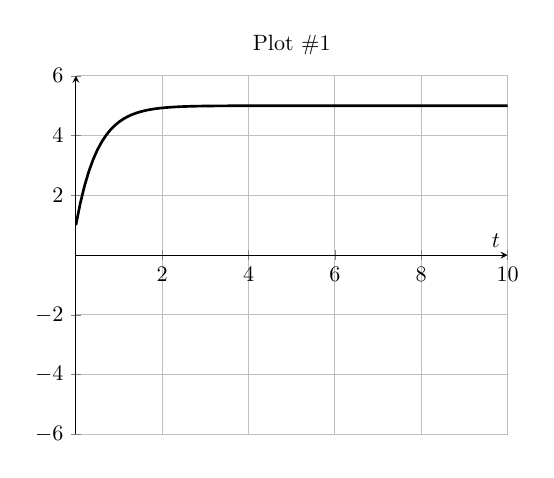
\begin{tikzpicture}[scale=\scl]
        \begin{axis}[axis lines=center, xlabel={$t$}, xmin=0, xmax=10, ymin=-6, ymax=6,
                grid, title={Plot \#1}]
                \addplot[very thick, domain=0:10, samples=100] {-4*exp(-2*x)+5};
        \end{axis}
    \end{tikzpicture}
    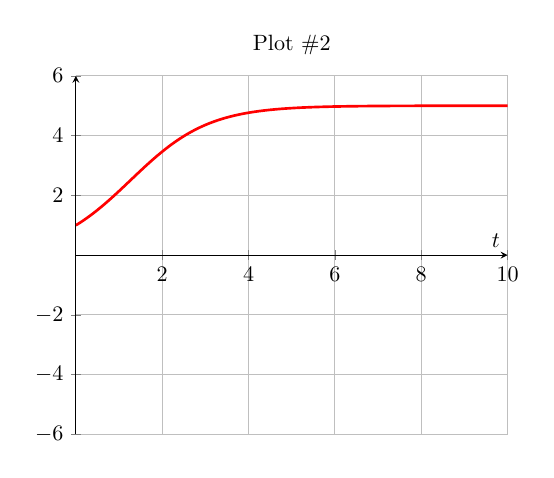
\begin{tikzpicture}[scale=\scl]
        \begin{axis}[axis lines=center, xlabel={$t$}, xmin=0, xmax=10, ymin=-6, ymax=6,
                grid, title={Plot \#2}]
                \addplot[very thick, domain=0:10, samples=150, color=red]
                {(5*exp(1.1*x))/(4+1*exp(1.1*x))};
        \end{axis}
    \end{tikzpicture}
\end{center}

\begin{center}
    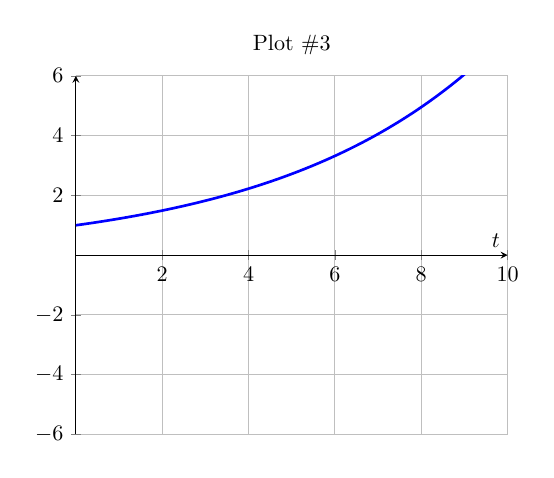
\begin{tikzpicture}[scale=\scl]
        \begin{axis}[axis lines=center, xlabel={$t$}, xmin=0, xmax=10, ymin=-6, ymax=6,
                grid, title={Plot \#3}]
                \addplot[very thick, domain=0:10, samples=100, color=blue] {exp(0.2*x)};
        \end{axis}
    \end{tikzpicture}
    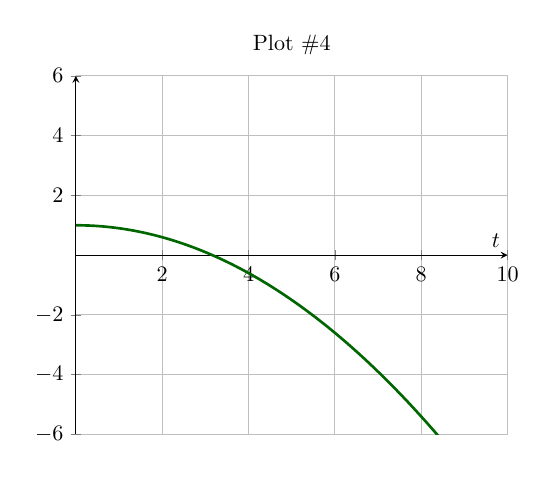
\begin{tikzpicture}[scale=\scl]
        \begin{axis}[axis lines=center, xlabel={$t$}, xmin=0, xmax=10, ymin=-6, ymax=6,
                grid, title={Plot \#4}]
                \addplot[very thick, domain=0:10, samples=100, color=green!40!black] {-0.1*x^2+1};
        \end{axis}
    \end{tikzpicture}
\end{center}
\end{problem}
\solution{
3,2,1,4. \\
Hint: Use what you know about the dynamics of the differential equations without solving
them.  For example, is there a steady state?  are there multiple steady states? etc.
}


\begin{problem}
    For each of the following scenarios write a differential equation and give an
appropriate initial condition.  Do not solve these differential
equations.
\begin{enumerate}
    \item[(a)] A tank contains 10kg of salt and 2000L of water.  Pure water enters the tank
    at a rate of 4L/min, the solution is thoroughly mixed, and solution is drained at 3
    L/min.  Let $S(t)$ be the amount of salt in the tank at time $t$.  Write a
    differential equation describing the amount of salt in the tank.
    \[ \frac{dS}{dt} = \underline{\hspace{2in}} \quad \text{with} \quad S(0) =
        \underline{\hspace{0.75in}} \]
        \solution{
            \[ \frac{dS}{dt} = -\frac{3S}{2000+1t} \quad \text{with} \quad S(0) = 10 \]
        }

    \item[(b)] Oil is pumped continuously from a well at a rate proportional to the amount
    of oil left in the well.  Initially there were 2 million barrels of oil in the well.
    Let $y(t)$ be the number is barrels left in the well (measured in millions of
    barrels).
    \vspace{0.1in} 
    \[ y' = \underline{\hspace{2in}} \quad \text{with} \quad y(0) =
        \underline{\hspace{0.75in}} \]
        \solution{
            $y'=-ky$ with $y(0) = 2$
        }
    \item[(c)] Newton's Law of Cooling states that the rate of change of the temperature
        of a cooling body (like tea in a cup) is proportional to the difference
        between the current temperature and the ambient room temperature.  Assume that the
        tea starts at 160$^\circ$F and cools, eventually, to 66$^\circ$F.  Write the
        differential equation associated with Newton's Law of Cooling.
        \[ \frac{dT}{dt} = \underline{\hspace{2in}} \quad \text{with} \quad T(0) =
            \underline{\hspace{0.75in}} \]
        \solution{
            \[ \frac{dT}{dt} = -k(T-66) \quad \text{with} \quad
                T(0) = 160 \]
        }
    \item[(d)] A pair of turtles, let's call them Adam and Eve, start a turtle colony in a
    small Montana pond (let's just ignore the lack of genetic diversity here).  The
    population of turtles in the pond follows these simple rules:  (1) If there
    are no turtles then the population clearly doesn't change, (2) the pond can support
    roughly 100 turtles, and (3) when the population is growing and is far away from the
    carrying capacity the growth rate is roughly proportional to the size of the
    population.  Let $P(t)$ be the size of the turtle population at time $t$.
    \[ \frac{dP}{dt} = \underline{\hspace{2in}} \quad \text{with} \quad S(0) =
        \underline{\hspace{0.75in}} \]
        \solution{
            \[ \frac{dP}{dt} = -kP\left( 1-\frac{P}{100} \right) \quad \text{with} \quad
                P(0) = 2 \]
        }

    \item[(e)] A 120-gallon tank initially contains 90 pounds of salt dissolved in 100
    gallons of water. Brine containing 2 pounds per gallon of salt flows into the tank at
    a rate of 4 gallons per minute and the well stirred mixture flows out of the tank at a
    rate of 3 gallons per minute (so the tank is filling up). Write a differential
    equation for the amount of salt in the tank.
    \[ \frac{dS}{dt} = \underline{\hspace{2in}} \quad \text{with} \quad S(0) =
        \underline{\hspace{0.75in}} \]
        \solution{
            \[ \frac{dS}{dt} = 8  -\frac{3S}{100+t} \quad \text{with} \quad y(0) = 10 \]
        }
\end{enumerate}
\end{problem}


\begin{problem}
    In Problem \ref{prob:ice_balls} we built models for the melting of ice cubes.  Solve
    both of the differential equations resulting from those models and answer the
    question: which type of ice cube will keep my drink colder longer.
\end{problem}
\begin{problem}
    A stone is dropped from rest at an initial height $h$ above the surface of the earth.
    We want to show that the speed with which it strikes the ground is $v = \sqrt{2gh}$.
    Start by writing an appropriate differential equation and then use the
    differential equation to very this result. You do not need to include air resistance
    in your model.
\end{problem}
\solution{
    \[ \frac{dv}{dt} = -g \implies v(t) = -gt + 0 \implies \frac{dy}{dt} = -gt \implies
    y(t) = -\frac{gt^2}{2} + h \implies t_{ground} =\sqrt{\frac{2h}{g}} \]
    Therefore,
    \[ v_{ground} = -g\sqrt{\frac{2h}{g}} = -\sqrt{2gh} \]
}

\begin{problem}
    In a local pine forest the Pine Beetle is killing the trees at a rate proportional to the
    number of available trees in the forest.  A conservation group is attempting to curb the
    problem by planting 5 live trees per week.  Write a differential equation describing
    this scenario, classify the differential equation, and determine if it can be solved
    with separation of variables.
%     Which of the following is a mathematical model
%     for the number of live trees as a function of time (measured in weeks)?
%     \begin{enumerate}
%         \item $T' = -kT + 5$
%         \item $T' = -kT + 5*t$
%         \item $T' = -5k*T*t$
%         \item $T' = -5k*t$
%     \end{enumerate}
\end{problem}
\solution{
$T' = -kT + 5$.  First order, linear, autonomous, non-homogeneous. Separation is fine
since is it autonomous.
\[ \int \frac{dT}{T-5/k} = \int -k dt = -kt+C \implies \ln(T-5/k) = -kt+C \implies T =
Ce^{-kt} + \frac{5}{k} \]
}


\begin{problem}
    In the movie Interstellar, ``Plan B'' was for the astronauts to start a colony on a new
    planet.  There was 1 female in the group so she would presumably carry the children.
    Genetic diversity was no problem because of the donor eggs.  The supplies on the colony
    would be limited by local resources as well as what they brought with them
    (which minimal).  Which of the following models should the astronauts use to plan
    their future reproduction, and what do the parameters mean?  Explain your choice for the best one.
    \begin{itemize}
        \item $P' = kP$
        \item $P' = kt$
        \item $P' = -kP\ln(P/N)$
        \item $P' = kP(1-P/N) $
    \end{itemize}
\end{problem}
\solution{A logistic model is the best choice. Either of the last two choice could work.
    \[ \int \frac{dP}{P\ln(P/N)} = \int -k dt \implies \int \frac{dP}{P\ln(P/N)} = -kt + C
    \]
    \[ \implies (\text{with } u=P/N) \,  \int \frac{1}{u\ln(u)} = -kt+C \implies
    (\text{with } v=1/u) \, \int \frac{1}{v}dv = -kt + C \]
    \[ \implies \ln(v) = -kt+c \implies \ln(\ln(P/N))=-kt+C \implies \ln(P/N) = Ce^{-kt}
    \implies P(t) = N e^{Ce^{-kt}} \]

    For the more standard logistic model:
    \[ \int \frac{dP}{P(1-P/N)} = -kt+C \implies \int \frac{A}{P} + \frac{B}{1-P/N} dP =
    -kt + C \implies \int \frac{1}{P} + \frac{(1/N)}{1-P/N} dP = -kt+ C \]
    \[ \implies \ln(P) - \ln(1-P/N) = -kt+C \implies \ln \left( \frac{P}{1-P/N} \right) =
    -kt+C\]
    \[ \implies \frac{P}{1-P/N} = Ce^{-kt} \implies P(t) = \frac{Ce^{-kt}}{1-Ce^{-kt}/N}
    \]

}


\begin{problem}
    Canyon Ferry reservoir has a volume of approximately $V = 2.33 \times 10^9$ m$^3$ and assume that the inflow from the
    Missouri river in the spring is $R=113$ m$^3$/sec.  Assume further
    that the dam leading to Hauser reservoir is open so the outflow rate is the same as
    the inflow rate in Canyon Ferry.  A large gas tank at a marina upstream is 
    leaking into the river so the contaminated water coming in has a concentration of
    $c = 0.25$kg/m$^3$.  
    Write a differential equation for the amount of gas, $G(t)$, in Canyon Ferry lake at
    time $t$.  Assume for simplicity that the gas is well mixed in the lake.  Once you
    have your model solve it with an appropriate technique. \\
    Hint \#1: The rate of change of the amount of gas equals the rate in minus the rate out
    \[ \frac{dG}{dt} = \text{rate that the gas comes in} - \text{rate that the gas goes
    out} \]
    Hint \#2: Do not substitute the values given until you have solved the model.
%     \begin{enumerate}
%         \item $\displaystyle \frac{dG}{dt} = 113 \cdot 2.33 \times 10^9 - \frac{113 \cdot
%             G}{0.25}$
%         \item $\displaystyle \frac{dG}{dt} = 113 \cdot 0.25 - \frac{113 \cdot G}{2.33 \times 10^9}$
%         \item $\displaystyle \frac{dG}{dt} = 113 \cdot 0.25 - \frac{2.33 \times 10^9 \cdot
%             G}{113}$
%         \item $\displaystyle \frac{dG}{dt} = 0.25 \cdot 2.33 \times 10^9 - \frac{113 \cdot
%             G}{0.25}$
%     \end{enumerate}
\end{problem}
\solution{
The correct model is:
\[ \frac{dG}{dt} = R \cdot c - \frac{R G}{V} \]
where $R$ is the flow rate, $c$ is the contamination concentration, $V$ is the volume of
the lake, and $G$ is the amount of gas in the water. Therefore, the correct model is
\[ \frac{dG}{dt} = 113 \cdot 0.25 - \frac{113 \cdot G}{2.33 \times 10^9} \]
The solution can be found either with separation, integrating factors, or with
undetermined coefficients. 
\[ \frac{dG}{dt} = -\frac{R}{V} \left( G - cV \right) \implies G(t) = Ce^{-Rt/V} + cV \]

Explore with slope fields.

Extension.  What if the rates are not the same and $V = V(t)$? Must use integrating
factors.

}

